% Copyright (c) 2018 Victorien Elvinger
% Code licensed under GPLv3 (https://www.gnu.org/licenses/gpl-3.0.en.html).
% Content licensed under CC-BY 4.0 (https://creativecommons.org/licenses/by/4.0/).

\documentclass[xcolor=table,t,french]{beamer}
% t: vertical flush of every frame (local override possible)

\usepackage[utf8]{inputenc}
\usepackage[french]{babel}

% Theme
% -----------
\usetheme[
    sectionpage=simple,
    numbering=fraction
]{metropolis}
\setbeamertemplate{title page}[default]
\setbeamercolor{palette primary}{bg=black!80}
\setbeamerfont{footnote}{size=\scriptsize}
\setbeamersize{text margin left=4.4ex, text margin right=4.4ex}

% Prelude
% -----------
\usepackage{acronym} % Acronyms \ac[p], \acl[p], \acs[p], \acf[p]

\acrodef{CRDT}[CRDT]{Conflict-free Replicated Data Type}
\acrodefplural{CRDT}[CRDTs]{Conflict-free Replicated Data Types}

\acrodef{poset}[poset]{partially ordered set}

\acrodef{VTNS}[VTNS]{Visibilité Transitive Non-Spéculative}

\acrodef{FJC}[FJC]{Fork-Join-Causal}
\acrodef{VFJC}[VFJC]{View-\acl{FJC}}
\acrodef{SVFJC}[SVFJC]{Stabilizable-\acl{VFJC}}

\acrodef{BFT}[BFT]{Byzantine Fault-Tolerant}

\acrodef{CS}[CS]{Causal Stability}
\acrodef{PCS}[PCS]{Provable \acl{CS}}
\acrodef{VFJCS}[VFJCS]{\acl{VFJC} Stability}

\acrodef{fjc}[fjc]{fork-join-causally}
\acrodef{vfjc}[vfjc]{view-\acl{fjc}}

\acrodef{cs}[cs]{causalement stable}
\acrodefplural{cs}[cs]{causalement stables}
\acrodef{pcs}[pcs]{provably \acl{cs}}
\acrodef{vfjcs}[vfjcs]{\acl{vfjc} stable}

\acrodef{MUTE}[MUTE]{Multi-User Text Editor}

\acrodef{RGA}[RGA]{Replicated Growable Array}

\usepackage[backend=biber,defernumbers=true,bibstyle=trad-plain,citestyle=authortitle,sorting=none,maxbibnames=1,maxcitenames=1]{biblatex}

\addbibresource{references/bft.bib}
\addbibresource{references/collaborative.bib}
\addbibresource{references/consistency.bib}
\addbibresource{references/crdt.bib}
\addbibresource{references/general.bib}
\addbibresource{references/publications.bib}

\AtBeginBibliography{\footnotesize}
\setbeamertemplate{bibliography item}[text] % use ref number in bibliography

\renewcommand{\thefootnote}{[\arabic{footnote}]}
    % Footnote style: [footnote-counter]

\newcommand\singlefootnote[1]{%
    % Use this footnote variant when a single footnote is on the page
    % Footnote style: *
    \begingroup
    %\renewcommand\thefootnote{}\footnote{#1}%
    \renewcommand{\thefootnote}{*}\footnote{#1}%
    \addtocounter{footnote}{-1}%
    \endgroup
}

% map defaulf block to oldblock
\let\oldblock\block
\let\endoldblock\endblock

% change block by adding smallskip
\renewenvironment{block}[1]
    {\begin{oldblock}{#1}
        \smallskip
    }
    { 
    \end{oldblock}
    }
\usepackage{color}

\definecolor{dirt}{HTML}{7A4A3B}
\definecolor{gold}{HTML}{B09500}
\definecolor{olive}{HTML}{82B366}
\definecolor{sky}{HTML}{72B1FF}
\definecolor{pumpkin}{HTML}{EB811B}
\definecolor{pinky}{HTML}{9673A6}

\definecolor{valid}{HTML}{82B366}
\definecolor{invalid}{HTML}{B85450}

%\colorlet{hl}{yellow!70!}
\colorlet{hl}{orange!30!}

\usepackage{graphicx}
\graphicspath{{./fig/}}

\usepackage{booktabs} % better tables

\usepackage{hyperref}

\newenvironment{compactitemize}{%
\settowidth{\leftmargini}{\usebeamertemplate{itemize item}}%
\addtolength{\leftmargini}{\labelsep}%
\begin{itemize}%
}{\end{itemize}}

\newenvironment{compactenumerate}{%
\settowidth{\leftmargini}{\usebeamertemplate{enumerate item}}%
\addtolength{\leftmargini}{\labelsep}%
\begin{enumerate}%
}{\end{enumerate}}
% Math
\usepackage{amsmath,amssymb}
\usepackage{mathtools} % fix amsmath bugs + better typeset

% Math - paired notations
% Each commands
% - has a * version that scales to the size of the content
%   e.g. set*{x}
% - an option to specify delimiter size
%   e.g. set[\Big]{x}
%   among: \big, \Big, \bigg, \Bigg

\DeclarePairedDelimiter{\tuple}{\langle}{\rangle}

\providecommand{\given{}}
\newcommand*{\setgivenpart}[1][]{%
    \nonscript\:#1\vert\allowbreak\nonscript\:\mathopen{}}
\DeclarePairedDelimiterX{\set}[1]{\{}{\}}{%
    \renewcommand\given{\setgivenpart[\delimsize]}#1}
\DeclarePairedDelimiterX{\setopen}[1]{\{}{.}{%
    \renewcommand\given{\setgivenpart[\delimsize]}#1}
\DeclarePairedDelimiterX{\setclose}[1]{.}{\}}{%
    \renewcommand\given{\setgivenpart[\delimsize]}#1}

\newcommand*{\trm}[1]{\operatorname{\mathsf{#1}}} % custom math term

\usepackage{pifont}

\newcommand{\xmark}{\ding{53}}

\usepackage{tikz}
\usetikzlibrary{arrows.meta} % '-latex' arrow
\usetikzlibrary{backgrounds}
\usetikzlibrary{fit} % fit attribute
\usetikzlibrary{positioning}
\usetikzlibrary{overlay-beamer-styles} % on <n>
\usetikzlibrary{calc} % for calculation
\usetikzlibrary{graphs}
\usetikzlibrary{quotes} % shortcut for labels
\usetikzlibrary{shapes.misc}

\usetikzlibrary{3d}
% https://tex.stackexchange.com/questions/48774/drawing-axis-grid-in-3d-with-custom-unit-vectors
\makeatletter
\tikzoption{canvas is xy plane at z}[]{%
  \def\tikz@plane@origin{\pgfpointxyz{0}{0}{#1}}%
  \def\tikz@plane@x{\pgfpointxyz{1}{0}{#1}}%
  \def\tikz@plane@y{\pgfpointxyz{0}{1}{#1}}%
  \tikz@canvas@is@plane%
}
\makeatother

\tikzset{>=latex}

\tikzset{
    link/.style = {dotted,line width=0.5mm},
    vis/.style = {-latex},
}


\tikzset{
    doc/.pic={
        \fill[scale=.1,fill=white,draw=gray,thick,solid] (0,0) -- (7,0) -- (7,8) -- (5,10) -- (0,10) -- cycle;
    },
    square/.pic={
        \fill[sky,scale=.1] (0,0) rectangle (3,3);
    },
    circle/.pic={
        \fill[scale=.05] (3,3) circle (3);
    },
    triangle/.pic={
        \fill[scale=.05] (0,0) -- (6,0) -- (3,6) -- cycle;
    },
    trapeze/.pic={
        \fill[scale=.05] (0,0) -- (6,1.5) -- (6,4.5) -- (0,6) -- cycle;
    },
}

\tikzset{
    compact/.style={inner sep=2,outer sep=1.85,rounded corners},
}

\tikzset{
    disabled/.style={opacity=.3},
    disabled on/.style={alt=#1{disabled}{}},
    fillhighlight/.style={fill=hl},
    fillhighlight on/.style={alt=#1{fillhighlight}{}},
    invisible/.style={opacity=0,text opacity=0},
    visible on/.style={alt={#1{}{invisible}}},
    on/.style 2 args={alt=#1{#2}{}},
}

\tikzset{
    stable/.style = {draw,rounded corners=0},
    stable on/.style={alt=#1{stable}{}}
}

\newcommand\lettersize{7.6mm}
\newcommand\biglettersize{8.7mm}
\newcommand\widthblock{15.2mm}

\tikzset{
    username/.style={below, font=\scriptsize, text width={width ("Alice")}, align=center},
    letter/.style={draw, minimum size=\lettersize, font=\ttfamily, node distance=\lettersize and \lettersize, on grid, label position=below},
    bigletter/.style={letter, minimum size=\biglettersize, node distance=\biglettersize and \biglettersize},
    block/.style={draw, minimum height=\lettersize, minimum width=\widthblock, node distance=\widthblock and \lettersize, on grid},
    crossed/.style={
        inner sep=.222em,
        path picture={
            \draw[red,thick] (path picture bounding box.west) -- (path picture bounding box.east);
        }
    }
}

% \newcommand{\ufcounter}[1]{
%     % 1: maximum count
%     \foreach[count=\counter] \i in {1,..., #1} {\only<\i|handeout:0>{\i}}
% }

% \newcommand{\ufcircledcounter}[2]{
%     % 1: position, 2: maximum count
%     \node[
%             fill,
%             circle,
%             text=white,
%             inner sep=1pt,
%             font=\scriptsize
%         ] at (#1) {\ufcounter{#2}};
% }

\usepackage{soul} % hl, st, ul
\setstcolor{red}
\sethlcolor{hl}

\renewcommand<>{\hl}[1]{\only#2{\beameroriginal{\hl}}{#1}}
\renewcommand<>{\so}[1]{\only#2{\beameroriginal{\so}}{#1}}
\renewcommand<>{\st}[1]{\only#2{\beameroriginal{\st}}{#1}}
\renewcommand<>{\ul}[1]{\only#2{\beameroriginal{\ul}}{#1}}

% https://tex.stackexchange.com/questions/41683/why-is-it-that-coloring-in-soul-in-beamer-is-not-visible
\makeatletter
\newcommand\SoulColor{%
  \let\set@color\beamerorig@set@color
  \let\reset@color\beamerorig@reset@color}
\makeatother
\SoulColor


%
\usebackgroundtemplate{%
\begin{tikzpicture}[opacity=0.3]
    \draw[step=3ex,gray,thin] (current page.south east) grid (current page.north west);
\end{tikzpicture}
}


\usepackage[scale=1.5]{ccicons}
\usepackage{transparent}

\usepackage{silence}
\WarningFilter{biblatex}{Patching footnotes failed}
    % Filter warning of biblatex package: "Patching footnotes failed"

\usepackage{appendixnumberbeamer}


% Meta-data
% ---------

\author{Victorien Elvinger}
\title{Réplication sécurisée dans les infrastructures pair-à-pair de collaboration}
\institute{%
    
\includegraphics[height=1.6em]{/logo/loria.pdf}\hspace{1.6em}%
    
\includegraphics[height=1.6em]{/logo/ul.pdf}\hspace{1.6em}%
    
\includegraphics[height=1.6em]{/logo/cnrs.pdf}\hspace{1.6em}%
    
\includegraphics[height=1.6em]{/logo/inria.pdf}\hspace{1.6em}%
    %\newline Supervisé par Dr. Gérald Oster et Prof. François Charoy%
}
\date{Juin 2021}


% Content
% -------
\includeonly{
    context,
    problematic-1,
    problematic-2,
    conclusion,
    backup,
}

\begin{document}

{ % Title page
    \metroset{numbering=none}
    \begin{frame}[c]
        \maketitle
        \center{
            \footnotesize%
            \begin{tabular}{rl}
                Membres du jury~: &\\
                Steve Kremer & directeur de recherche Inria Grand Est\\
                Emmanuelle Anceaume & directrice de recherche IRISA\\
                Pascal Molli & professeur à l'Université de Nantes\\
                Esther Pacitti & professeure à l'Université de Montpellier 2\\
                François Charoy & professeur à l'Université de Lorraine\\
                Gérald Oster & maître de conférence à l'Université de Lorraine\\
            \end{tabular}
        }
    \end{frame}
}


% {
% \usebackgroundtemplate{%
%   \parbox[c][\paperheight][c]{\paperwidth}{\centering
\includegraphics[width=0.9\paperwidth]{collab/world-map.pdf}}
% }
% \begin{frame}{Activités de collaboration}

% \end{frame}
% }


\begin{frame}{Applications de collaboration}
    \begin{minipage}[c][.55\textheight][t]{\textwidth}
        \centering
        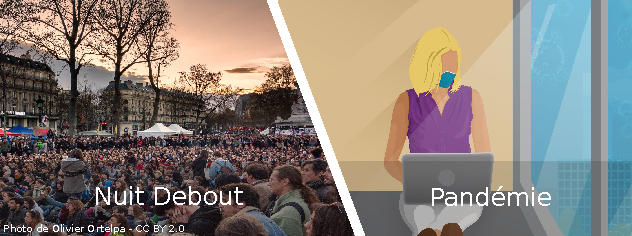
\includegraphics[width=\textwidth]{collab/collab-activity.pdf}
    \end{minipage}
    \begin{minipage}{\textwidth}
        \begin{compactitemize}
            \item plusieurs individus \textbf{modifient ensemble} un contenu
            \begin{compactitemize}
                \item localisés à des \textbf{endroits différents}
                \item modifications en \textbf{simultané} ou à des \textbf{moments distincts}
            \end{compactitemize}
            \item \textbf{collaborations massives}
            \begin{compactitemize}
                \item met en lumière les limites des applications existantes
            \end{compactitemize}
        \end{compactitemize}
    \end{minipage}
\end{frame}

\begin{frame}{Infrastructure centralisée de collaboration}
    \begin{minipage}[c][.55\textheight][t]{\textwidth}
        \centering
        \begin{tikzpicture}
            \newcommand*\sep{2.8}
            % devices
            \node[
                label=below:{Serveur·s}
            ](S){
\includegraphics[scale=.5]{collab/cloud.pdf}};
            \path (S)
                +(30:\sep) node[
                    "Alice" below,
                ](A){
\includegraphics[scale=.35]{collab/device.pdf}}
                +(-30:\sep) node[
                    "Bea" below,
                ](B){
\includegraphics[scale=.35]{collab/device.pdf}}
                +(180:\sep) node[
                    "Carol" below,
                ](C){
\includegraphics[scale=.35]{collab/device.pdf}};
            % Links
            \node(doc)[anchor=south,inner sep=.111em] at (S.north){
                \tikz[scale=.05]{
                    \pic {doc};
                    \pic<2->[fill=sky] at (1,13) {square};
                    \pic<2->[fill=olive] at (7,8) {circle};
                }
            };
            \only<1>{
                \graph[edges={link}]{
                    {(A.west), (B.west)} -> (S),
                    (C) -- (S)
                };
                \path (A.west) -- node[pos=.33]{
                    \tikz\pic[fill=sky]{square};
                } (S);
                \path (B.west) -- node[pos=.33]{
                    \tikz\pic[fill=olive]{circle};
                } (S);
            }
            \only<2>{
                \node{
\includegraphics[scale=.4]{collab/sync.pdf}};
                \graph[edges={link}]{
                    {(A.west), (B.west), (C)} -- (S)
                };
            }
            \only<3>{
                \graph[
                    edges={link},
                    edge node={
                        node{
                            \tikz[scale=.05]{
                                \pic {doc};
                                \pic[fill=sky] at (1,13) {square};
                                \pic[fill=olive] at (7,8) {circle};
                            }
                        }
                    },
                ]{
                    (S) -> {(A.west), (B.west), (C)}
                };
            }
            \only<4>{ % availability
                \node{\color{invalid} \xmark};
            }
            \only<5>{ % content property
                \draw[invalid,very thick] (doc.north west) -- (doc.south east);
                \graph[edges={link}]{
                    {(A.west), (B.west), (C)} -- (S)
                };
            }
            \only<6>{ % scalability
                \node[anchor=south] at (S.base){
                    
\includegraphics[scale=.12]{collab/fire.pdf}
                };
                \path (S)
                    +(150:\sep) node(D){
\includegraphics[scale=.35]{collab/device.pdf}}
                ;
                \graph[edges={link}]{
                    {[
                        edge node={
                            node[pos=.33]{
                                \tikz\pic[fill=sky]{square};
                            }
                        }
                    ](A.west) -> (S)},
                    {[
                        edge node={
                            node[pos=.33]{
                                \tikz\pic[fill=olive]{circle};
                            }
                        }
                    ](B.west) -> (S)},
                    {[
                        edge node={
                            node[pos=.33]{
                                \tikz\pic[fill=pinky]{triangle};
                            }
                        }
                    ](C) -> (S)},
                    {[
                        edge node={
                            node[pos=.33]{
                                \tikz\pic[fill=gold]{trapeze};
                            }
                        }
                    ](D.east) -> (S)},
                };
            }
            \only<7>{ % security & privacy
                \node{
\includegraphics[scale=.2]{collab/eye.pdf}};
                \graph[edges={link}]{
                    {(A.west), (B.west), (C)} -- (S)
                };
            }
            \only<8>{ % offline
                \graph[edges={link}]{
                    (S) -- {(A.west), (B.west)}
                };
                \node[anchor=base] at (C.north){
                    
\includegraphics[scale=.02]{collab/nowifi.pdf}
                };
            }
        \end{tikzpicture}
    \end{minipage}
    \begin{minipage}[c][4ex][t]{\textwidth}
        {\color{pumpkin} \textbf{Limites}}
    \end{minipage}
    \begin{minipage}{\textwidth}
        \begin{minipage}{.38\textwidth}
            \begin{compactitemize}
                \item disponibilité
                \item latence
                \item sécurité et vie privée
            \end{compactitemize}
        \end{minipage}
        \begin{minipage}{.58\textwidth}
            \begin{compactitemize}
                \item propriété des contenus
                \item passage à l'échelle
                \item modes de collaboration (hors ligne)
            \end{compactitemize}
        \end{minipage}
    \end{minipage}
\end{frame}

\begin{frame}{Infrastructures pair-à-pair de collaboration}
    \begin{minipage}[c][.55\textheight][t]{\textwidth}
        \centering
        \begin{tikzpicture}
                \newcommand*\sep{1.5}
                \newcommand*\ang{80}
                % devices
                \path (0,0)
                +(\ang:\sep) node[
                    "Alice",
                    label=right:{%
                        \tikz[scale=.05]{
                            \pic {doc};
                            \pic[fill=sky] at (1,13) {square};
                            \pic<3- |handout:0>[fill=olive] at (7,8) {circle};
                            \pic<4- |handout:0>[fill=pinky] at (7,1) {triangle};
                        }
                    },
                ](A){
\includegraphics[scale=.35]{collab/device.pdf}}
                +(\ang-120:\sep) node[
                    "Bea" below,
                    label=right:{%
                        \tikz[scale=.05]{
                            \pic {doc};
                            \pic<3- |handout:0>[fill=sky] at (1,13) {square};
                            \pic[fill=olive] at (7,8) {circle};
                            \pic<4- |handout:0>[fill=pinky] at (7,1) {triangle};
                        }
                    },
                ](B){
\includegraphics[scale=.35]{collab/device.pdf}}
                +(\ang+120:\sep) node[
                    "Carol" below,
                    label=left:{%
                        \tikz[scale=.05]{
                            \pic {doc};
                            \pic<4- |handout:0>[fill=sky] at (1,13) {square};
                            \pic<4- |handout:0>[fill=olive] at (7,8) {circle};
                            \pic[fill=pinky] at (7,1) {triangle};
                        }
                    },
                ](C){
\includegraphics[scale=.35]{collab/device.pdf}}
            ;
            % Links
            \draw[link] (A) -- node[midway]{\includegraphics<2 | handout:0>[scale=.4]{collab/sync.pdf}} (B);
            \draw<3- | handout:0>[link] (B) -- node[midway]{\includegraphics<3 | handout:0>[scale=.4]{collab/sync.pdf}} (C);
            \draw<3- | handout:0>[link] (C) -- node[midway]{\includegraphics<3 | handout:0>[scale=.4]{collab/sync.pdf}} (A);
        \end{tikzpicture}
    \end{minipage}
    \begin{minipage}{\textwidth}
        \begin{compactitemize}
            %\item les pairs exécutent des \textbf{operations} pour modifier le contenu
            \item les pairs possèdent leur \textbf{propre copie} du contenu
            \begin{compactitemize}
                \item modifiable à \textbf{tout moment} et \textbf{sans coordination}
                \item \textbf{convergence à terme}
            \end{compactitemize}
            \item la convergence des copies est une propriété essentielle
        \end{compactitemize}
    \end{minipage}
\end{frame}


% \begin{frame}{Problématiques}
%     \begin{minipage}[c][.6\textheight][t]{\textwidth}
%         \centering
%         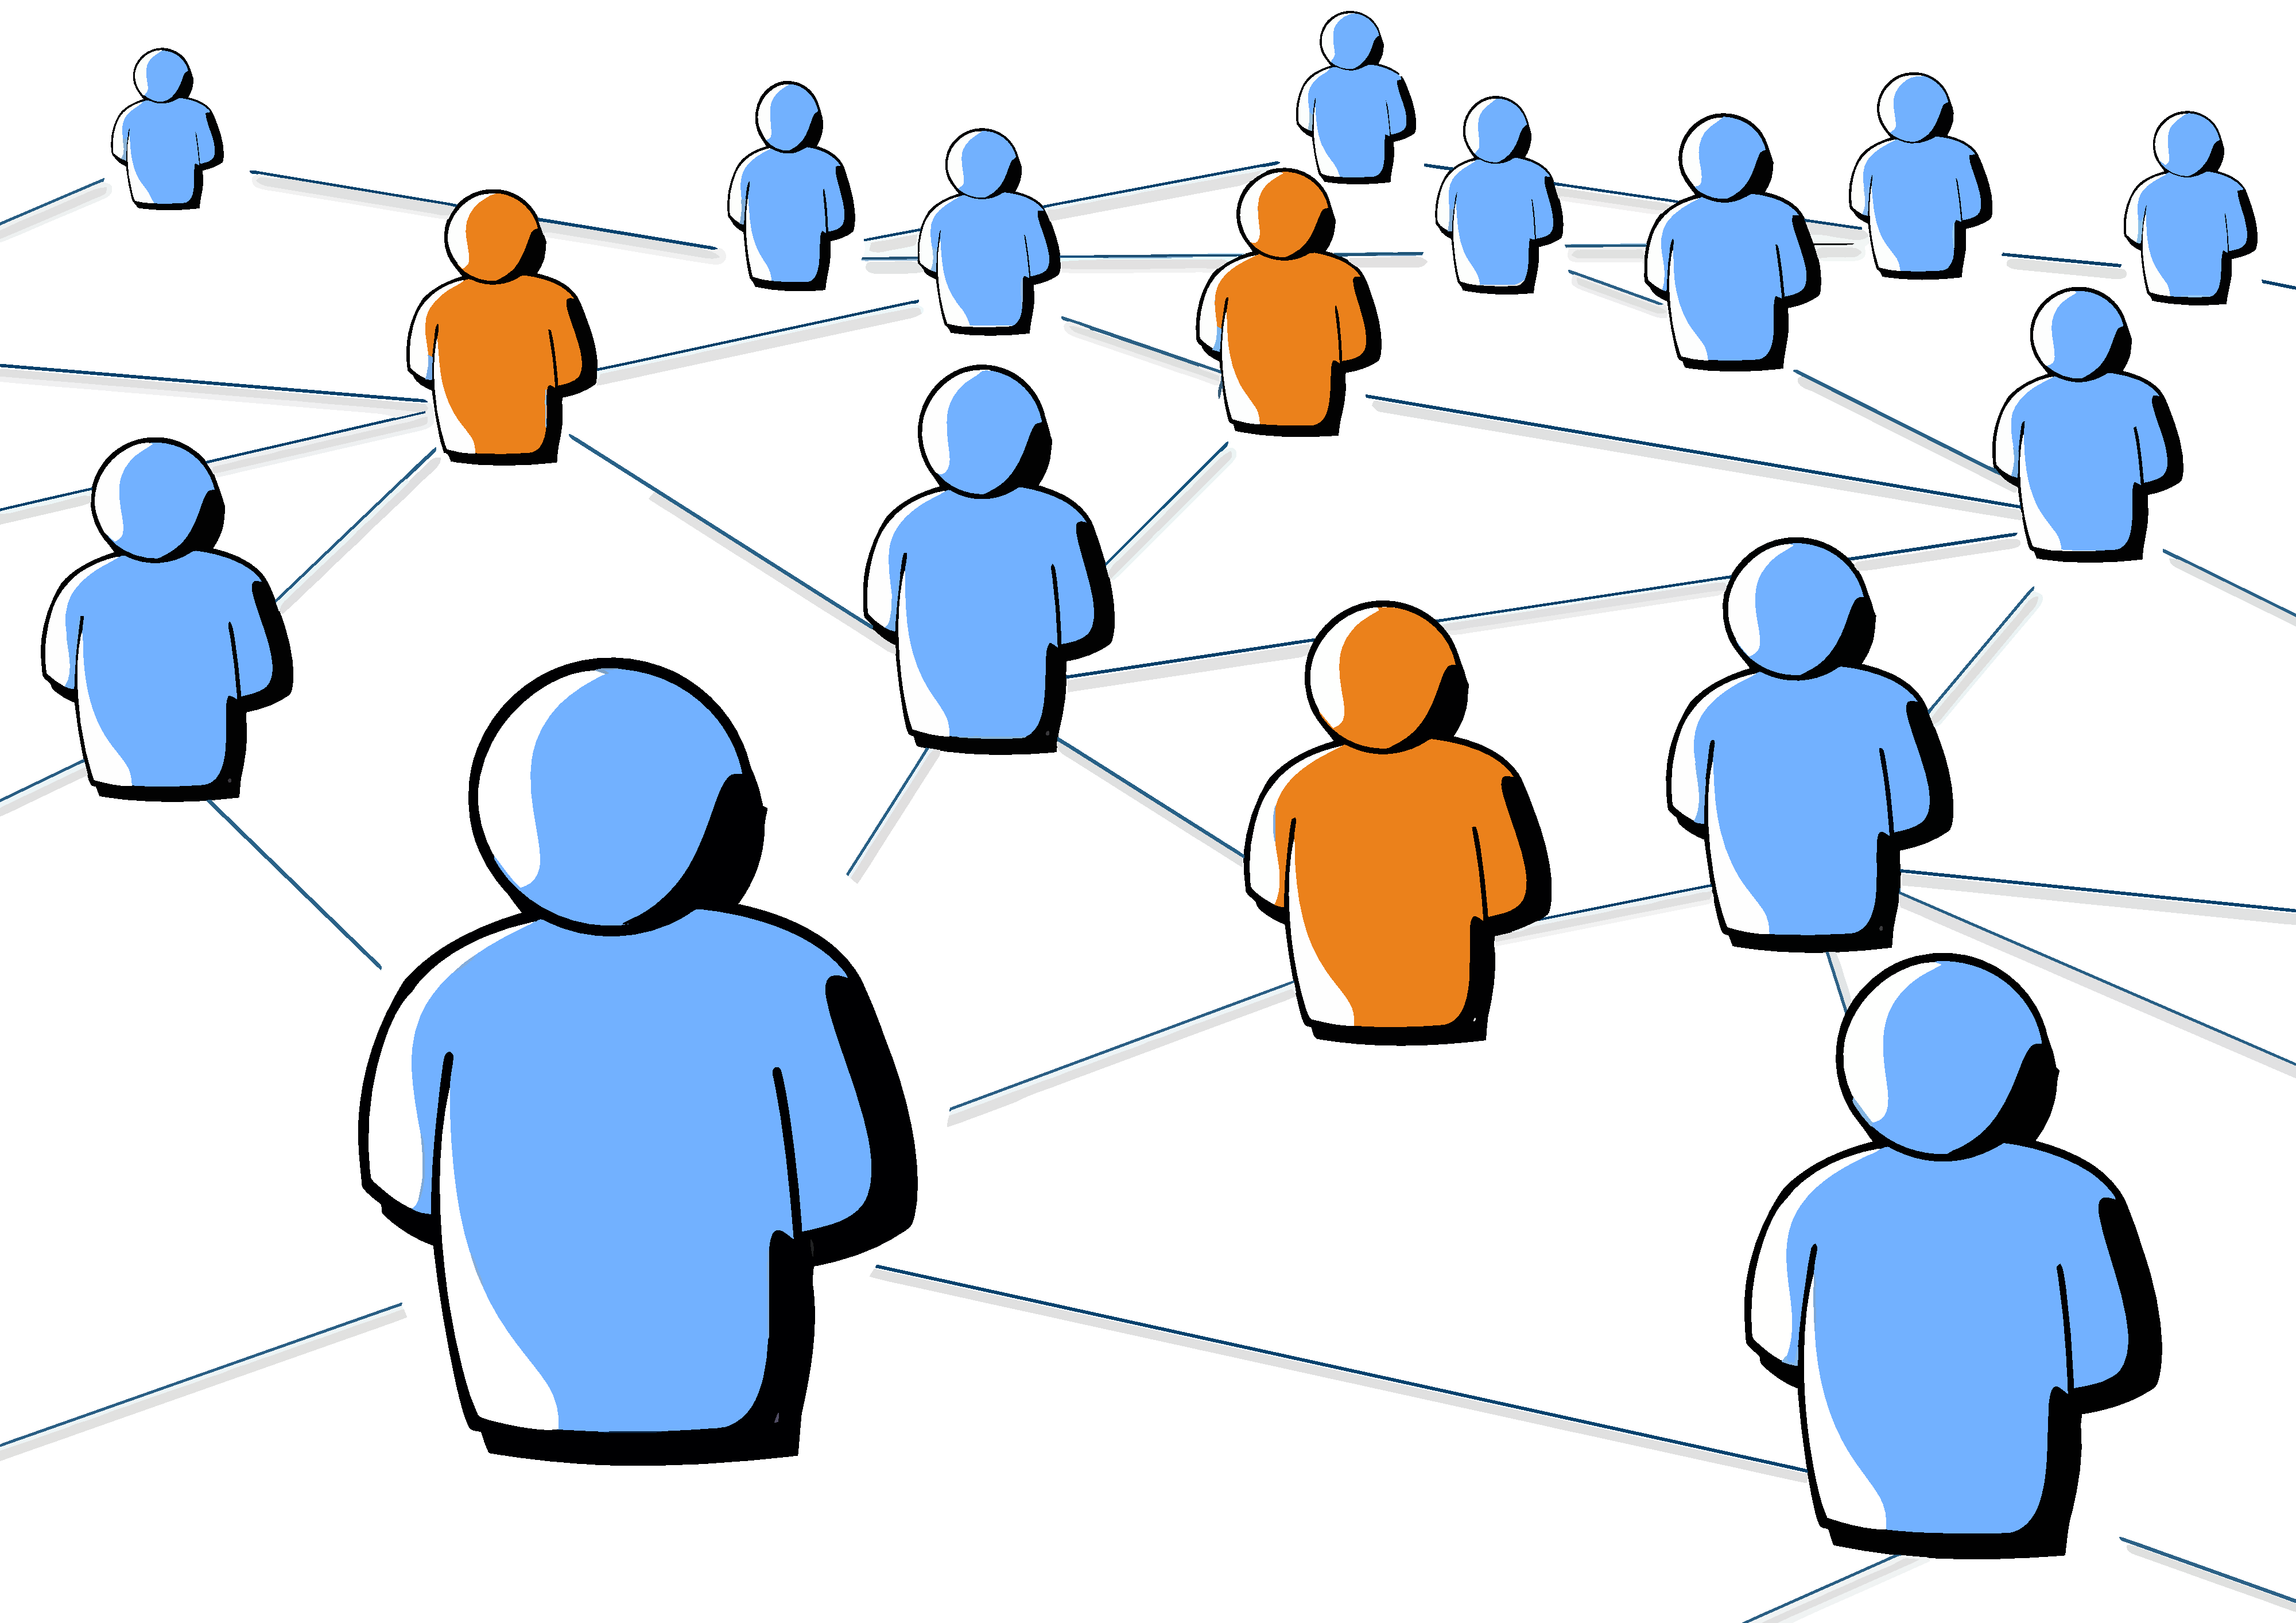
\includegraphics[scale=.1]{fig/materials/p2p.pdf}
%     \end{minipage}
%     \begin{minipage}{\textwidth}
%         \begin{compactitemize}
%             \item les pairs ont plus de responsabilités
%             \begin{compactitemize}
%                 \item ils peuvent plus facilement nuire à la collaboration
%             \end{compactitemize}
%             \item participation d'un plus grand nombre de collaborateur·ice·s
%             \begin{compactitemize}
%                 \item produit de nouveaux obstacles de passage à l'échelle
%             \end{compactitemize}
%         \end{compactitemize}
%     \end{minipage}
% \end{frame}


\begin{frame}[plain,standout]
    Problématique 1~: peut-on\\assurer la convergence des copies\\ en présence de pairs malintentionnés~?\\
    \vspace{2em}
    Problématique 2~:\\peut-on concevoir un protocole pour la co-édition de texte qui résiste mieux aux aléas du réseau et aux longues périodes de déconnexion~?\\
\end{frame}



{ % Problematic 1
    % \setbeamercolor{palette primary}{
    %     bg=dirt
    % }
    \begin{frame}[plain,standout]
    Problématique 1~: peut-on\\assurer la convergence des copies\\ en présence de pairs malintentionnés~?\\
    \vspace{2em}
    \begin{tikzpicture}
        \node[
            label=below:{\normalsize Mallory},
        ] {
\includegraphics[scale=.806]{collab/evil-cat.pdf}};
    \end{tikzpicture}
\end{frame}


\begin{frame}{Qu'est ce qu'un pair malintentionné~?}
    \begin{minipage}[c][.55\textheight][t]{\textwidth}
        \centering
        \begin{tikzpicture}
            \newcommand*\sep{1.5}
            \newcommand*\ang{80}
            % devices
            \path (0,0)
                +(\ang:\sep) node[
                    "Alice",
                    label={[shift={(-1,0)},opacity=0]right:{%
                        
\includegraphics[scale=0.4]{collab/log-sample.pdf}%
                    }},
                    label=right:{%
                        \tikz[scale=.05]{
                            \pic {doc};
                            \pic[fill=sky] at (1,13) {square};
                            \pic[fill=olive] at (7,8) {circle};
                            \pic<2-3>[fill=pumpkin] at (7,1) {triangle};
                        }
                    },
                ](A){
\includegraphics[scale=0.35]{collab/device.pdf}}
                +(\ang-120:\sep) node[
                    "Bea" below,
                    label=right:{%
                        \tikz[scale=.05]{
                            \pic {doc};
                            \pic[fill=sky] at (1,13) {square};
                            \pic[fill=olive] at (7,8) {circle};
                            \pic<2-3>[fill=pumpkin] at (1,1) {trapeze};
                        }
                    },
                ](B){
\includegraphics[scale=0.35]{collab/device.pdf}}
                +(\ang+120:\sep) node[
                    "Mallory" below
                ](M){
\includegraphics[scale=.35]{collab/evil-cat.pdf}};
            % Links
            \draw[link] (A) -- node[midway]{\includegraphics<2>[scale=0.4]{collab/sync.pdf}} (B);
            \draw<1>[link,->] (M) -> node[pos=.33]{\tikz\pic[fill=pumpkin]{triangle};} (A);
            \draw<1>[link,->] (M) -> node[pos=.33]{\tikz\pic[fill=pumpkin]{trapeze};} (B);
            \draw<2->[link] (M) -- (A);
            \draw<2->[link] (M) -- (B);
        \end{tikzpicture}
    \end{minipage}
    \begin{minipage}{\textwidth}
        \begin{compactitemize}
            \item adversaire de la collaboration
            \begin{compactitemize}
                \item objectif~: \textbf{empêcher la convergence} des copies
                \item \emph{Byzantin}~: \textbf{pairs malintentionnés + réseau asynchrone corrompu}
            \end{compactitemize}
            \item un pair malintentionné peut compromettre la convergence par \textbf{équivoques} = modifications distinctes perçues comme identiques
        \end{compactitemize}
    \end{minipage}
\end{frame}


\begin{frame}{Journaux de modifications}
    \begin{minipage}[c][.55\textheight][t]{\textwidth}
        \centering
        \begin{tikzpicture}
            \newcommand*\sep{1.5}
            \newcommand*\ang{80}
            % devices
            \node(A) at (\ang:\sep)[
                "Alice",
                label=right:{%
                    \tikz[scale=.05]{
                        \pic<2-> {doc};
                        \pic<4->[fill=sky] at (1,13) {square};
                        \pic<5->[fill=olive] at (7,8) {circle};
                        \pic<6->[fill=pumpkin] at (7,1) {triangle};
                        %\pic<8->[fill=pumpkin] at (1,1) {trapeze};
                    }
                },
            ]{
\includegraphics[scale=0.35]{collab/device.pdf}};
            \node(B) at (\ang-120:\sep)[
                "Bea" below,
                label=right:{%
                    \tikz[scale=.05]{
                        \pic<3-> {doc};
                        \pic<5->[fill=sky] at (1,13) {square};
                        \pic<4->[fill=olive] at (7,8) {circle};
                        %\pic<8->[fill=pumpkin] at (7,1) {triangle};
                        \pic<6->[fill=pumpkin] at (1,1) {trapeze};
                    }
                },
            ]{
\includegraphics[scale=0.35]{collab/device.pdf}};
            \node(M) at (\ang+120:\sep)[
                "Mallory" below
            ]{
\includegraphics[scale=0.35]{collab/evil-cat.pdf}};
            % Logs

            \newcommand{\opDoc}{\tikz[x=1cm,y=1cm]\pic[scale=.4,fill=sky]{doc};}
            \newcommand{\opSq}{\tikz[x=1cm,y=1cm]\pic[fill=sky]{square};}
            \newcommand{\opCirc}{\tikz[x=1cm,y=1cm]\pic[fill=olive]{circle};}
            \newcommand{\opTri}{\tikz[x=1cm,y=1cm]\pic[fill=pumpkin]{triangle};}
            \newcommand{\opTra}{\tikz[x=1cm,y=1cm]\pic[fill=pumpkin]{trapeze};}

            \node[
                "\scriptsize journal de Alice",
                right=1.4 of A.north east,
                anchor=north west,
                draw,
                dashed,
                text width=5.9cm,
            ]{\begin{tikzpicture}[
                    node distance=.8cm and 1.3cm,
                    on grid
                ]
                \visible<2->{\node(new) {\opDoc};}
                \node<4->(sq)[right=of new] {\opSq};
                \node<5->(circ)[right=of sq] {\opCirc};
                \node<6->(tri)[right=of circ] {\opTri};
            \end{tikzpicture}};
            \node[
                "\scriptsize journal de Bea",
                right=1.4 of B.north east,
                anchor=north west,
                draw,
                dashed,
                text width=5.9cm,
            ]{\begin{tikzpicture}[node distance=.8cm and 1.3cm, on grid]
                \visible<3->{\node(new) {\opDoc};}
                \node<4->(circ)[right=of new] {\opCirc};
                \node<5->(sq)[right=of circ] {\opSq};
                \node<6->(tra)[right=of sq] {\opTra};
            \end{tikzpicture}};
            % Links
            \begin{scope}[every path/.style=link]
            \draw<1,3,5-> (A) -- (B);
            \draw<2>[->] (A) -> node[pos=.33]{\opDoc} (B);
            \draw<4>[->] (A) to[bend right=10] node[pos=.33]{\opSq} (B);
            \draw<4>[->] (B) to[bend right=10] node[pos=.33]{\opCirc} (A);

            \draw<1,3,6-> (A) -- (M);
            \draw<2>[->] (A) -> node[pos=.33]{\opDoc} (M);
            \draw<4>[->] (A) -> node[pos=.33]{\opSq} (M);
            \draw<5>[->] (M) -> node[pos=.33]{\opTri} (A);

            \draw<1-3,6-> (B) -- (M);
            \draw<4>[->] (B) -> node[pos=.33]{\opCirc} (M);
            \draw<5>[->] (M) -> node[pos=.33]{\opTra} (B);
            \end{scope}
        \end{tikzpicture}
    \end{minipage}
    \begin{minipage}{\textwidth}
        \begin{compactitemize}
            \item un pair enregistre dans son journal les \textbf{modifications qu'il intègre}
            \item arrangement horizontal $=$ ordre d'ajout des modifications
        \end{compactitemize}
    \end{minipage}
\end{frame}


\begin{frame}{Journaux infalsifiables}
    \begin{minipage}[c][.55\textheight][t]{\textwidth}
        \centering
        \begin{tikzpicture}
            \newcommand*\sep{1.5}
            \newcommand*\ang{80}
            % devices
            \node(A) at (\ang:\sep)[
                "Alice",
                label=right:{%
                    \tikz[scale=.05]{
                        \pic{doc};
                        \pic[fill=sky] at (1,13) {square};
                        \pic[fill=olive] at (7,8) {circle};
                        \pic[fill=pumpkin] at (7,1) {triangle};
                        \pic<4->[fill=pumpkin] at (1,1) {trapeze};
                    }
                },
            ]{
\includegraphics[scale=0.35]{collab/device.pdf}};
            \node(B) at (\ang-120:\sep)[
                "Bea" below,
                label=right:{%
                    \tikz[scale=.05]{
                        \pic{doc};
                        \pic[fill=sky] at (1,13) {square};
                        \pic[fill=olive] at (7,8) {circle};
                        \pic<4->[fill=pumpkin] at (7,1) {triangle};
                        \pic[fill=pumpkin] at (1,1) {trapeze};
                    }
                },
            ]{
\includegraphics[scale=0.35]{collab/device.pdf}};
            \node(M) at (\ang+120:\sep)[
                "Mallory" below
            ]{
\includegraphics[scale=0.35]{collab/evil-cat.pdf}};
            % Logs

            \newcommand{\opDoc}{\tikz[x=1cm,y=1cm]\pic[scale=.4,fill=sky]{doc};}
            \newcommand{\opSq}{\tikz[x=1cm,y=1cm]\pic[fill=sky]{square};}
            \newcommand{\opCirc}{\tikz[x=1cm,y=1cm]\pic[fill=olive]{circle};}
            \newcommand{\opTri}{\tikz[x=1cm,y=1cm]\pic[fill=pumpkin]{triangle};}
            \newcommand{\opTra}{\tikz[x=1cm,y=1cm]\pic[fill=pumpkin]{trapeze};}

            \node[
                "\scriptsize journal de Alice",
                right=1.4 of A.north east,
                anchor=north west,
                draw,
                dashed,
                text width=5.9cm,
                clabel/.style={font=\scriptsize,inner sep=0,anchor=south},
            ]{\begin{tikzpicture}[
                    node distance=.8cm and 1.3cm,
                    on grid
                ]
                \only<1-4>{
                    \node(a1) {\opDoc};
                    \node(a2)[right=of a1] {\opSq};
                }
                \only<1,2>{
                    \node(b1)[right=of a2] {\opCirc};
                    \node(m1)[right=of b1] {\opTri};
                }
                \only<3,4>{
                    \node(b1)[below right=of a2] {\opCirc};
                    \node(m1)[above right=of b1] {\opTri};
                }
                \only<2-4>{
                    \node[clabel] at (a1.south east) {A};
                    \node[clabel] at (a2.south east) {A};
                    \node[clabel] at (b1.south east) {B};
                    \node[clabel] at (m1.south east) {M};
                }
                \only<5>{
                    \node(a1) {$a_1$};
                    \node(a2)[right=of a1] {$a_2$};
                    \node(b1)[below right=of a2] {$b_1$};
                    \node(m1)[above right=of b1] {$m_1$};
                    \node(m1p)[below right=of m1] {$m_1'$};
                }
                \only<4>{
                    \node(m1p)[below right=of m1] {\opTra};
                    \node[clabel] at (m1p.south east) {M};
                }
                \only<3>{
                    \graph[edges={solid}]{
                        (a1) -> {
                            (a2) -> (m1),
                            (b1)
                        }
                    };
                }
                \only<4->{
                    \graph[edges={solid}]{
                        (a1) -> {
                            (a2) -> (m1),
                            (b1) -> (m1p)
                        }
                    };
                }
            \end{tikzpicture}};
            \node[
                "\scriptsize journal de Bea",
                right=1.4 of B.north east,
                anchor=north west,
                draw,
                dashed,
                text width=5.9cm,
                clabel/.style={font=\scriptsize,inner sep=0,anchor=south},
            ]{\begin{tikzpicture}[node distance=.8cm and 1.3cm, on grid]
                \only<1-4>{
                    \node(a1) {\opDoc};
                    \node(b1)[right=of a1] {\opCirc};
                }
                \only<1,2>{
                    \node(a2)[right=of b1] {\opSq};
                    \node(m1p)[right=of a2] {\opTra};
                }
                \only<3,4>{
                    \node(a2)[below right=of b1] {\opSq};
                    \node(m1p)[above right=of a2] {\opTra};
                }
                \only<2-4>{
                    \node[clabel] at (a1.south east) {A};
                    \node[clabel] at (a2.south east) {A};
                    \node[clabel] at (b1.south east) {B};
                    \node[clabel] at (m1p.south east) {M};
                }
                \only<5>{
                    \node(a1) {$a_1$};
                    \node(b1)[right=of a1] {$b_1$};
                    \node(a2)[below right=of b1] {$a_2$};
                    \node(m1p)[above right=of a2] {$m_1'$};
                    \node(m1)[below right=of m1p] {$m_1$};
                }
                \only<4>{
                    \node(m1)[below right=of m1p] {\opTri};
                    \node[clabel] at (m1.south east) {M};
                }
                \only<3>{
                    \graph[edges={solid}]{
                        (a1) -> {
                            (b1) -> (m1p),
                            (a2)
                        }
                    };
                }
                \only<4->{
                    \graph[edges={solid}]{
                        (a1) -> {
                            (a2) -> (m1),
                            (b1) -> (m1p)
                        }
                    };
                }
            \end{tikzpicture}};
            % Links
            \graph[edges={link}]{(A) -- (B) -- (M), (A) -- (M)};
            \path<3> (A) -- node[midway]{
\includegraphics[scale=0.4]{collab/sync.pdf}} (B);
        \end{tikzpicture}
    \end{minipage}
    \begin{minipage}{\textwidth}
        \begin{compactitemize}
            \item \textbf{modifications signées} par leur auteur·ice
            \item \textbf{déclaration infalsifiable des dépendances} à l'aide de \textbf{\textit{hashes}}
            \begin{compactitemize}
                \item un pair malintentionné peut déclarer des dépendances arbitraires
            \end{compactitemize}
            \item journaux avec \textbf{mêmes modifications} $\implies$ \textbf{copies convergentes}
        \end{compactitemize}
    \end{minipage}
\end{frame}


\begin{frame}{Surcoût des journaux}
    \begin{minipage}[c][.6\textheight][t]{\textwidth}
        \centering
        \begin{tikzpicture}
            \newcommand*\sep{1.5}
            \newcommand*\ang{80}
            % devices
            \node(A) at (\ang:\sep)[
                "Alice",
                label=right:{%
                    \tikz[scale=.05]{
                        \pic {doc};
                        \pic[fill=sky] at (1,13) {square};
                        \pic[fill=olive] at (7,8) {circle};
                        \pic[fill=pumpkin] at (7,1) {triangle};
                        \pic[fill=pumpkin] at (1,1) {trapeze};
                    }
                },
                label={[shift={(1,0)}]right:{%
                    
\includegraphics[scale=0.4]{collab/log-sample.pdf}%
                }},
            ]{
\includegraphics[scale=0.35]{collab/device.pdf}};
            \node(B) at (\ang-120:\sep)[
                "Bea" below,
                label=right:{%
                    \tikz[scale=.05]{
                        \pic {doc};
                        \pic[fill=sky] at (1,13) {square};
                        \pic[fill=olive] at (7,8) {circle};
                        \pic[fill=pumpkin] at (7,1) {triangle};
                        \pic[fill=pumpkin] at (1,1) {trapeze};
                    }
                },
                label={[shift={(1,0)}]right:{%
                    
\includegraphics[scale=0.4]{collab/log-sample.pdf}%
                }},
            ](B){
\includegraphics[scale=0.35]{collab/device.pdf}};
            \coordinate(Cp) at (\ang+60:\sep*3);
            \node(C) at (Cp |- A)[
                "Carol" below,
                label=left:{%
                    \only<3>{
                        \tikz[scale=.05]{
                            \pic {doc};
                            \pic[fill=sky] at (1,13) {square};
                            \pic[fill=olive] at (7,8) {circle};
                            \pic[fill=pumpkin] at (7,1) {triangle};
                            \pic[fill=pumpkin] at (1,1) {trapeze};
                        }
                    }
                },
                label={[shift={(-1,0)},visible on=<2->]left:{%
                    
\includegraphics[scale=0.4]{collab/log-sample.pdf}%
                }},
            ]{
\includegraphics[scale=0.35]{collab/device.pdf}};
            % Links
            \draw[link] (A) -- (B);
            \draw<1>[link,->] (B) -> node[midway]{
\includegraphics[scale=0.3]{collab/log-sample.pdf}} (C);
            \draw<2->[link] (B) -- (C);
        \end{tikzpicture}
    \end{minipage}
    \begin{minipage}{\textwidth}
        \begin{description}
            \item[mémoire~:] les pairs conservent leur journal
            \item[communication~:] un nouveau pair récupère un journal
            \item[calcul~:] un nouveau pair intègre chaque modification
        \end{description}
        % Passage à l'échelle
        % Confidentialité
    \end{minipage}
\end{frame}


\begin{frame}{Que font les applications de collaboration~?}
    \begin{minipage}[c][.55\textheight][t]{\textwidth}
        \centering
        \begin{tikzpicture}
            \newcommand*\sep{1.5}
            \newcommand*\ang{80}
            % devices
            \node(A) at (\ang:\sep)[
                    "Alice",
                    label=right:{%
                        \tikz[scale=.05]{
                            \pic {doc};
                            \pic[fill=sky] at (1,13) {square};
                            \pic[fill=olive] at (7,8) {circle};
                            \pic[fill=pumpkin] at (7,1) {triangle};
                            \pic[fill=pumpkin] at (1,1) {trapeze};
                        }
                    },
                    label={[shift={(1,0)}]right:{%
                        
\includegraphics[scale=0.4]{collab/log-sample.pdf}%
                    }},
                ]{
\includegraphics[scale=0.35]{collab/device.pdf}};
                \node(B) at (\ang-120:\sep)[
                    "Bea" below,
                    label=right:{%
                        \tikz[scale=.05]{
                            \pic {doc};
                            \pic[fill=sky] at (1,13) {square};
                            \pic[fill=olive] at (7,8) {circle};
                            \pic[fill=pumpkin] at (7,1) {triangle};
                            \pic[fill=pumpkin] at (1,1) {trapeze};
                        }
                    },
                    label={[shift={(1,0)},visible on=<1>]right:{%
                        
\includegraphics[scale=0.4]{collab/log-sample.pdf}%
                    }},
                    label={[shift={(1,0)}, visible on=<2->]right:{%
                        
\includegraphics[scale=0.4]{collab/pruned-log.pdf}%
                    }},
                ]{
\includegraphics[scale=0.35]{collab/device.pdf}};
                \coordinate(Cp) at (\ang+60:\sep*3);
                \node(C) at (Cp |- A)[
                    "Carol",
                    label={[visible on=<4>]left:{%
                        \tikz[scale=.05]{
                            \pic {doc};
                            \pic[fill=sky] at (1,13) {square};
                            \pic[fill=olive] at (7,8) {circle};
                            \pic[fill=pumpkin] at (7,1) {triangle};
                            \pic[fill=pumpkin] at (1,1) {trapeze};
                        }
                    }},
                ]{
\includegraphics[scale=0.35]{collab/device.pdf}};
            % Links
            \draw[link] (A) -- (B);
            \draw<3>[link,->] (B) -> node[midway]{
                \tikz[scale=.05]{
                    \pic {doc};
                    \pic[fill=sky] at (1,13) {square};
                    \pic[fill=olive] at (7,8) {circle};
                    \pic[fill=pumpkin] at (7,1) {triangle};
                    \pic[fill=pumpkin] at (1,1) {trapeze};
                }
            } (C);
            \draw<4>[link] (B) -- (C);
        \end{tikzpicture}
    \end{minipage}
    \begin{minipage}{\textwidth}
        \begin{compactitemize}
            \item hypothèse~: taille contenu $<$ taille journal
            \item \textbf{troncature} du journal \textbf{sans coordination}
            \item \textbf{transmission de l'état de la copie} aux nouveaux pairs
        \end{compactitemize}
    \end{minipage}
\end{frame}


\begin{frame}{Diffucltés en présence de pairs malintentionnés}
    \begin{minipage}[c][.55\textheight][t]{\textwidth}
        \centering
        \begin{tikzpicture}
            \newcommand*\sep{1.5}
            \newcommand*\ang{80}
            % devices
            \node(A) at (\ang:\sep)[
                    "Alice",
                ]{
\includegraphics[scale=0.35]{collab/device.pdf}};
            \node(B) at (\ang-120:\sep)[
                "Bea" below,
            ]{
\includegraphics[scale=0.35]{collab/device.pdf}};
            \coordinate(Cp) at (\ang+60:\sep*3);
            \node(C) at (Cp |- A)[
                "Carol",
            ]{
\includegraphics[scale=0.35]{collab/device.pdf}};
            \node(M) at (\ang+120:\sep)[
                "Mallory" below
            ]{
\includegraphics[scale=0.35]{collab/evil-cat.pdf}};
            % Links
            \draw[link] (A) -- node[midway]{\includegraphics<1>[scale=0.4]{collab/sync.pdf}} (B) -- (M) -- (A);
            \draw<3>[link,->] (M) -> node[midway]{
                \tikz[scale=.05]{
                    \pic {doc};
                    \pic[fill=pumpkin] at (7,1) {triangle};
                }
            } (C);
            \draw<4->[link] (M) -- (C);
            \draw<4,5>[link] (A) -- node[midway]{\includegraphics<4>[scale=0.4]{collab/sync.pdf}} (C);
            % docs
            \node also[
                label=right:{%
                    \tikz[scale=.05]{
                        \pic {doc};
                        \pic[fill=sky] at (1,13) {square};
                        \pic[fill=olive] at (7,8) {circle};
                        \pic[fill=pumpkin] at (7,1) {triangle};
                        %\pic[fill=pumpkin] at (1,1) {trapeze};
                    }
                },
                label={[shift={(1,0)}]right:{%
                    
\includegraphics[scale=0.4]{collab/pruned-log.pdf}%
                }},
            ](A);
            \node also[
                label=right:{%
                    \tikz[scale=.05]{
                        \pic {doc};
                        \pic[fill=sky] at (1,13) {square};
                        \pic[fill=olive] at (7,8) {circle};
                        %\pic[fill=pumpkin] at (7,1) {triangle};
                        \pic[fill=pumpkin] at (1,1) {trapeze};
                    }
                },
                label={[shift={(1,0)}]right:{%
                    
\includegraphics[scale=0.4]{collab/pruned-log.pdf}%
                }},
            ](B);
            \node also[
                label={[visible on=<4->]left:{%
                    \tikz[scale=.05]{
                        \pic {doc};
                        \pic[fill=pumpkin] at (7,1) {triangle};
                    }
                }},
            ](C);
        \end{tikzpicture}
    \end{minipage}
    \begin{minipage}{\textwidth}
        \begin{compactitemize}
            \item le journal \textbf{ne peut pas être tronqué arbitrairement}
            \begin{compactitemize}
                \item la détection d'équivoque pourrait être compromise
            \end{compactitemize}
            \item un pair malintentionné peut transmettre un \textbf{état falsifié}
        \end{compactitemize}
    \end{minipage}
\end{frame}


\begin{frame}{Notre approche}
    \begin{minipage}[c][.55\textheight][t]{\textwidth}
        \centering
        \begin{tikzpicture}[x radius=2cm]
            \newcommand*\sep{1.5}
            \newcommand*\ang{80}
            % devices
            \node(A) at (\ang:\sep)[
                "Alice",
            ]{\includegraphics[scale=0.35]{collab/device.pdf}};
            \node(B) at (\ang-120:\sep)[
                "Bea" below,
            ]{\includegraphics[scale=0.35]{collab/device.pdf}};
            \coordinate(Cp) at (\ang+60:\sep*3);
            \node(C) at (Cp |- A)[
                "Carol" below,
            ]{\includegraphics[scale=0.35]{collab/device.pdf}};
            % Links
            \draw[link] (A) -- (B);
            \draw<1>[link, ->] (B) ->%
                    node[midway,above]{\includegraphics[scale=0.3]{collab/pruned-log.pdf}}%
                    node[midway,below]{
                        \tikz[scale=.05]{
                            \pic {doc};
                            \pic[fill=sky] at (1,13) {square};
                            \pic[fill=olive] at (7,8) {circle};
                            \pic[fill=pumpkin] at (7,1) {triangle};
                            \pic[fill=pumpkin] at (1,1) {trapeze};
                        }
                    }%
                (C);
            \draw<2->[link] (B) -- (C);
            % docs
            \node also[
                label=right:{%
                    \tikz[scale=.05]{
                        \pic {doc};
                        \pic[fill=sky] at (1,13) {square};
                        \pic[fill=olive] at (7,8) {circle};
                        \pic[fill=pumpkin] at (7,1) {triangle};
                        \pic[fill=pumpkin] at (1,1) {trapeze};
                    }
                },
                label={[shift={(1,0)}]right:{%
                    \includegraphics[scale=0.4]{collab/log-sample.pdf}%
                }},
            ](A);
            \node also[
                label=right:{%
                    \tikz[scale=.05]{
                        \pic {doc};
                        \pic[fill=sky] at (1,13) {square};
                        \pic[fill=olive] at (7,8) {circle};
                        \pic[fill=pumpkin] at (7,1) {triangle};
                        \pic[fill=pumpkin] at (1,1) {trapeze};
                    }
                },
                label={[shift={(1,0)}]right:{%
                    \includegraphics[scale=0.4]{collab/pruned-log.pdf}%
                }},
            ](B);
            \node also[
                label={[visible on=<2->]left:{%
                    \tikz[scale=.05]{
                        \pic {doc};
                        \pic[fill=sky] at (1,13) {square};
                        \pic[fill=olive] at (7,8) {circle};
                        \pic[fill=pumpkin] at (7,1) {triangle};
                        \pic[fill=pumpkin] at (1,1) {trapeze};
                    }
                }},
                label={[shift={(-1,0)},visible on=<2->]left:{%
                    \includegraphics[scale=0.4]{collab/pruned-log.pdf}%
                }},
            ](C);
        \end{tikzpicture}
    \end{minipage}
    \begin{minipage}{\textwidth}
        \begin{compactitemize}
            \item \textbf{troncature sans coordination} reposant sur le concept de \textbf{stabilité}
            \begin{compactitemize}
                \item conservation de modifications pour la détection d'équivoques
            \end{compactitemize}
            \item transmission d'un \textbf{état authentifiable} et journal tronqué
            \begin{compactenumerate}
                \item vérifie la cohérence du journal tronqué
                \item authentifie le contenu à partir du journal
            \end{compactenumerate}
        \end{compactitemize}
    \end{minipage}
\end{frame}


\begin{frame}{Journal causal}
    \begin{minipage}[c][.48\textheight][t]{\textwidth}
        \begin{tikzpicture}[x=1.3cm,y=.8cm,every node/.style={compact}]
            \node at (0,.9) {};
            \begin{scope}
                \node(A)["Alice" username] at (-1,0) {
                    \includegraphics[scale=.35]{collab/device.pdf}
                };
                \node(a1)[
                    fillhighlight on=<{1,7}>,
                ] at (0,0) {$a_1$};
                \node(a2)[
                    disabled on={<1>},
                    fillhighlight on=<{2,7}>,
                ] at (1,0) {$a_2$};
                \node(b1)[
                    disabled on=<1-2>,
                    fillhighlight on=<8>,
                ] at (2,-1) {$b_1$};
                \node[
                    disabled on=<1-2>,
                    fillhighlight on=<{3,7}>,
                ] (a3) at (3,0) {$a_3$};
                \graph{
                    (a1) ->[disabled on=<1>] (a2),
                    (a1) ->[disabled on=<1-2>] (b1),
                    {(a2), (b1)} ->[disabled on=<1-2>] (a3)
                };
            \end{scope}
            \begin{scope}[shift={(0,-2cm)}]
                \node(B)["Bea" username] at (-1,0) {
                    \includegraphics[scale=.35]{collab/device.pdf}
                };
                \node(a1)[
                    fillhighlight on=<7>,
                ] at (0,0) {$a_1$};
                \node(b1)[
                    fillhighlight on=<{4,8}>,
                ] at (1,0) {$b_1$};
                \node(a2)[
                    disabled on=<4>,
                    fillhighlight on=<6-7>,
                ] at (2,-1) {$a_2$};
                \node[
                    disabled on=<4>,
                    fillhighlight on=<6-7>,
                ] (a3) at (3,0) {$a_3$};
                \node(b2)[
                    disabled on=<4>,
                    fillhighlight on=<{5-6,8}>,
                ] at (4,0) {$b_2$};
                \graph[edges={disabled on=<4>}]{
                    (a1) -> {
                        (a2),
                        (b1)
                    },
                    (b1) ->[visible on=<{1-5,7-}>] (a3) ->[visible on=<{1-5,7-}>] (b2),
                    (a2) -> (a3)
                };
                \draw<6>[->] (b1) to[bend left=15] (b2);
                \node<6> at (b2.east)[anchor=west]{\color{invalid} \xmark};
            \end{scope}
        \end{tikzpicture}
    \end{minipage}
    \begin{minipage}{\textwidth}
        \textbf{Invariants}
        \begin{compactenumerate}
            \item {\only<7->{\transparent{.6}}une modification du possesseur du journal dépend des précédentes}
            \item {\only<-6>{\transparent{.6}}ordre linéaire des modification de chaque pair}
        \end{compactenumerate}
        % \begin{compactitemize}
        %     \item le possesseur du journal observe toutes les modifications
        %     \item les dépendances traduisent les observations des autres pairs
        % \end{compactitemize}
    \end{minipage}
\end{frame}


\begin{frame}{Stabilité causale}
    \begin{minipage}[c][.48\textheight][t]{\textwidth}
        \begin{tikzpicture}[x=1.3cm,y=.8cm,every node/.style={compact}]
            \node at (0,.9) {};
            \begin{scope}
                \node["Alice" username] at (-1,0) {
                    \includegraphics[scale=0.35]{collab/device.pdf}
                };
                \node(a1)[
                    stable on=<2->,
                ] at (0,0) {$a_1$};
                \node(a2)[
                    stable on=<5->,
                ] at (1,0) {$a_2$};
                \node(b1)[
                    fillhighlight on=<1>,
                    stable on=<2->,
                ] at (2,-1) {$b_1$};
                \node(a3)[
                    stable on=<5->,
                ] at (3,0) {$a_3$};
                \graph{
                    (a1) -> {(a2), (b1)} -> (a3)
                };
                \only<1>{
                    \node(b2) at (4,0) {$b_2$};
                    \graph[edges={dashed}]{
                        (a3) ->["?"] (b2),
                        (b1) ->["?" below] (b2)
                    };
                }
                \only<5>{
                    \node(b2)[
                        stable,
                    ] at (4,0) {$b_2$};
                    \graph{
                        (a3) -> (b2)
                    };
                }
            \end{scope}
            \begin{scope}[shift={(0,-2cm)}]
                \node at (0,.9) {};
                \node["Bea" {below,username}, "x" {opacity=0,username}] at (-1,0) {
                    \includegraphics[scale=0.35]{collab/device.pdf}
                };
                \node(a1)[
                    stable on=<4->,
                ] at (0,0) {$a_1$};
                \node(b1)[
                    stable on=<4->,
                ] at (1,0) {$b_1$};
                \node(a2)[
                    stable on=<4->,
                ] at (2,-1) {$a_2$};
                \node(a3)[
                    fillhighlight on=<3>,
                    stable on=<4->,
                ] at (3,0) {$a_3$};
                \node(b2) at (4,0) {$b_2$};
                \graph{
                    (a1) -> {(a2), (b1)} -> (a3) -> (b2)
                };
            \end{scope}
        \end{tikzpicture}
    \end{minipage}
    \begin{minipage}{\textwidth}
        \begin{definition}
            modification stable $\iff$ dépendance de toute modification \textbf{ultérieurement acceptée} dans le journal.
        \end{definition}
        \begin{theorem}
            modification stable $\iff$ observée par chaque pair au sein du journal.
        \end{theorem}
    \end{minipage}
\end{frame}


\begin{frame}{Jounal \acf{VFJC}}
    \begin{minipage}[c][.3\textheight][t]{\textwidth}
        \begin{tikzpicture}[x=1.3cm,y=.8cm,every node/.style={compact}]
            \node at (0,.9) {};
            \node(A)["Alice" username] at (-1,0) {
                \includegraphics[scale=0.35]{collab/device.pdf}
            };
            \node(a1) at (0,0) {$a_1$};
            \node(m1)[
                fillhighlight on=<1>,
                disabled on=<3>,
            ] at (1,0) {$m_1$};
            \node(b1)at (2,-1) {$b_1$};
            \node(a2)[disabled on=<3>]  at (3,0) {$a_2$};
            \node(m1p)[
                fillhighlight on=<{1,5}>,
                disabled on=<2>,
            ] at (4,-1) {$m_1'$};
            \node(b2)[
                disabled on=<2>,
                "\color{invalid} \xmark" {right, visible on=<4>},
            ] at (5,-1) {$b_2$};
            \node(a3)[
                "$\scriptstyle\set*{M}$" {visible on=<5>},
                disabled on=<2-4>,
            ] at (6,0) {\includegraphics[scale=.15]{collab/eye.pdf}};
            \graph{
                (a1) ->[disabled on=<3>] (m1) ->[disabled on=<3>] (a2),
                (a1) -> (b1),
                (b1) ->[disabled on=<3>] (a2),
                (b1) ->[disabled on=<2>] (m1p) ->[disabled on=<2>] (b2),
                {(a2), (b2)} ->[disabled on=<2-4>] (a3),
                (a2) ->[visible on=<4>] (b2)
            };
        \end{tikzpicture}
    \end{minipage}
    \begin{minipage}{\textwidth}
        \textbf{Invariants}
        \begin{compactenumerate}
            \item {\transparent{.6}une modification du possesseur du journal dépend des précédentes}
            \item {\transparent{.6}ordre linéaire des modification de chaque pair honnête}
            \item une modification \textbf{dépend directement} de modifications \textbf{présumées linéaires}
            \begin{compactitemize}
                \item {\only<1-4>{\transparent{.6}}une modification non-linéaire est acceptée indirectement}
                \item {\only<1-4>{\transparent{.6}}le possesseur du jorunal ne peut plus accepter directement de modifications d'un pair reconnu malintentionné}
            \end{compactitemize}
        \end{compactenumerate}
    \end{minipage}
\end{frame}


\begin{frame}{Stabilité et invariants de journaux}
    \begin{tikzpicture}[every node/.append style={
        align=center,
        inner sep=.5em,
    },node distance=.3cm and 1.6cm]
        \node(honest){environnement\\honnête};
        \node(malicious)[right=of honest]{environnement\\malintentionné};
        \node(static)[below left=of honest]{groupe\\statique};
        \node(dyn)[below=of static]{groupe\\dynamique};

        \node(causal)[below=of honest]{journal causal\footcite{hutto_1990_causal}\\stabilité causale\footcite{baquero_2018_pure-op-crdt}};
        \node(vfjc)[below=of malicious]{journal VFJC\footcite{mahajan_2011_cac}\\ \textbf{stabilité VFJC}};
        \node(dyncausal)[below=of causal]{\textbf{journal DynCausale}\\ \textbf{stabilité DynCausale}};
        \node(dynvfjc)[below=of vfjc]{\textbf{journal DynVFJC}\\ \textbf{stabilité DynVFJC}};

        \draw[thick] (dyn.west |- honest.south) -- (malicious.south -| dynvfjc.east);
        \draw[thick] (honest.north -| dyn.east) -- (dyn.south east);
    \end{tikzpicture}
    groupe statique = groupe avec un ensemble défini de pairs\\
    groupe dynamique = groupe dont la composition évolue
\end{frame}


\begin{frame}{Journal \acs{VFJC}}
    \begin{minipage}[c][.5\textheight][t]{\textwidth}
        \begin{tikzpicture}[x=1.3cm,y=.8cm,every node/.style={compact}]
            \node at (0,1.7) {};
            \node["Alice" username] at (-1,0) {
                \includegraphics[scale=0.35]{collab/device.pdf}
            };
            \node(a1)[
                fillhighlight on=<1>,
                "\scriptsize stable~?" {below, visible on=<1>},
            ] at (0,0) {$a_1$};
            \node(m1) at(1,0) {$m_1$};
            \node(b1) at (2,-1) {$b_1$};
            \node(a2) at(3,0) {$a_2$};
            \node<2>(m1p) at (4,-2) {$m_1'$};
            \node<2>(b2) at (5,-1) {$b_2$};
            \node<3>(b1p) at (4,1) {$b_1'$};
            \node<3>(m2) at (5,1) {$m_2$};
            \node(a3) at (6,0) {\includegraphics[scale=.15]{collab/eye.pdf}};
            \graph{
                (a1) -> (m1) -> (a2) -> (a3),
                (a1) -> (b1) -> (a2),
            };
            \only<2>{
                \graph{
                    (b1) -> (b2) -> (a3),
                    (m1p) -> (b2),
                };
            }
            \only<3>{
                \graph{
                    (m1) ->[bend left=25] (m2),
                    (b1p) -> (m2) -> (a3),
                };
            }
        \end{tikzpicture}
    \end{minipage}
    \begin{minipage}{\textwidth}
        \begin{compactitemize}
            \item le possesseur du journal \textbf{présume honnêtes} les autres pairs
            \begin{compactitemize}
                \item il s'attend à ce qu'ils soient \textbf{potentiellement malintentionnés}
            \end{compactitemize}
        \end{compactitemize}
    \end{minipage}
\end{frame}


\begin{frame}{Contribution~: Stabilité \acs{VFJC}}
    \newcommand{\eye}{\includegraphics[scale=.15]{collab/eye.pdf}}
    \begin{minipage}[c][.3\textheight][t]{\textwidth}
        \begin{tikzpicture}[x=1.3cm,y=-.8cm,every node/.style={compact}]
            \node at (0,.9) {};
            \node["Alice" username] at (-1,0) {
                \includegraphics[scale=0.35]{collab/device.pdf}
            };
            \node(a1)[stable] at (0,0) {$a_1$};
            \node(m1) at(1,0) {$m_1$};
            \node(a2) at(2,0) {$a_2$};
            \node(b1)[stable] at (3,1) {$b_1$};
            \node(m1p)[stable] at (4,1) {$m_1'$};
            \node(b2) at (5,1) {$b_2$};
            \node[
                "$\scriptstyle\set*{M}$"
            ] (a3) at (6,0) {\eye};
            \graph{
                (a1) -> (m1) -> (a2),
                (a1) -> (b1) -> (m1p) -> (b2),
                {(a2), (b2)} -> (a3)
            };
        \end{tikzpicture}
    \end{minipage}
    \begin{minipage}{\textwidth}
        \centering
        \begin{tabular}{cc}
            permutation & chaîne de dépendance\\
            \toprule
            $M, B, A$ & $m_1', b_2, \eye$\\
            $B, M, A$ & $b_2, \eye, \eye$\\
        \end{tabular}
    \end{minipage}
    \begin{minipage}{\textwidth}
        \begin{theorem}
            modification $x$ stable $\iff$ pour toute permutation $p_1, \dotsc, p_N$ des pairs avec $p_N$ le possesseur du journal, il existe une chaîne de dépendances $x, x_1, \dotsc, x_N$ telle que $x_i$ a pour auteur ou reconnaît malintentionné $p_i$.
        \end{theorem}
    \end{minipage}
\end{frame}


\begin{frame}{Contribution~: Jounal causal dynamique}
    \begin{minipage}[c][.3\textheight][t]{\textwidth}
        \begin{tikzpicture}[x=1.33cm,y=.8cm,every node/.style={compact}]
            \node at (0,.9) {};
            \node["Alice" username] at (-1,0) {
                \includegraphics[scale=0.35]{collab/device.pdf}
            };
            \node(a1)[
                fillhighlight on=<3>,
                "$\scriptstyle\trm{invit}({A,B})$"{
                    fillhighlight on=<{1,3}>,
                },
            ] at (0,0) {$a_1$};
            \node(a2)[
                fillhighlight on=<3>,
            ] at (1,0) {$a_2$};
            \node(b1)[
                fillhighlight on=<1>,
                "$\scriptstyle\trm{invit}(C)$"{
                    below,
                    fillhighlight on=<2>%
                },
            ] at (2,-1) {$b_1$};
            \node(c1)[
                fillhighlight on=<2>,
            ] at (3,0) {$c_1$};
            \node(b2)[
                fillhighlight on=<1>,
            ] at (4,0) {$b_2$};
            \graph{
                (a1) -> {(a2), (b1)} -> (c1) -> (b2)
            };
        \end{tikzpicture}
    \end{minipage}
    \begin{minipage}{\textwidth}
        \begin{compactitemize}
            \item suivi de la composition du groupe via les invitations
            \item les modifications d'un pair dépendent des dépendances de son invit.
        \end{compactitemize}
        \medskip
        \textbf{Invariants}
        \begin{compactenumerate}
            \item {\transparent{.6}une modification du possesseur du journal dépend des précédentes}
            \item {\transparent{.6}ordre linéaire des modifications de chaque pair}
            \item les modifications d'un pair dépendent de son invitation
        \end{compactenumerate}
    \end{minipage}
\end{frame}


\begin{frame}{Contribution~: Stabilité causale dynamique}
    \begin{minipage}[c][.3\textheight][t]{\textwidth}
        \begin{tikzpicture}[x=1.3cm,y=.8cm,every node/.style={compact}]
            \node at (0,.9) {};
            \node["Alice" username] at (-1,0) {
                \includegraphics[scale=0.35]{collab/device.pdf}
            };
            \node(a1)[
                stable,
                fillhighlight on=<1>,
                "$\scriptstyle\trm{invit}({A,B})$"{
                    fillhighlight on=<2->,
                },
            ] at (0,0) {$a_1$};
            \node(a2)[
                stable on=<6->,
                fillhighlight on=<{2,3,5-6}>,
            ] at (1,0) {$a_2$};
            \graph{
                (a1) -> (a2)
            };
            \only<3->{
                \node(b1)[
                    stable,
                    fillhighlight on=<4>,
                    "$\scriptstyle\trm{invit}(C)$"{
                        fillhighlight on=<{3,5-}>,
                        below,
                    },
                ] at (2,-1) {$b_1$};
                \graph{
                    (a1) -> (b1)
                };
            }
            \only<5->{
                \node(c1)[
                    stable on=<6->,
                    fillhighlight on=<5-6>,
                ] at (3,0) {$c_1$};
                \graph{
                    {(a2), (b1)} -> (c1)
                };
            }
            \only<6->{
                \node(b2)[
                    fillhighlight on=<7>,
                ] at (4,0) {$b_2$};
                \graph{
                    (c1) -> (b2)
                };
            }
        \end{tikzpicture}
    \end{minipage}
    \begin{minipage}{\textwidth}
        \begin{compactitemize}
            \item observateurs honnêtes requis =
            \begin{compactitemize}
                \item[+] pairs invités dans les dépendances
                \item[+] pairs invités en concurrence
            \end{compactitemize}
    \end{compactitemize}
    \end{minipage}
    \begin{minipage}{\textwidth}
        % \begin{tabular}{ccc}
        %     $a_2$ & $a_3, c_1, b_2$ & $b_1$ \\
        %     \toprule
        %     $\set*{A}$ & $\set*{A, B}$ & $\set*{A, B}$ \\
        %     $\emptyset$ & $\set*{C}$ & $\emptyset$ \\
        % \end{tabular}
    \end{minipage}
    \begin{minipage}{\textwidth}
        \begin{theorem}
            modification stable $\iff$ elle est observée par chacun de ses observateurs honnêtes requis au sein du journal.
        \end{theorem}
    \end{minipage}
\end{frame}


\begin{frame}{Résumé des contributions}
    \begin{compactitemize}
        \item contributions
        \begin{compactitemize}
            \item formalisation et généralisation du \textbf{concept de stabilité}
            \item formalisation des journaux et leurs invariants
            \item protocole à \textbf{journaux complets} et protocole à \textbf{journaux tronqués}
            \item formalisation et preuves des garanties offertes par les protocoles
            \item \textbf{algorithme à complexité linéaire}\singlefootnote{par rapport à la taille du journal} pour déterminer un sous-ensemble de modifications stables
        \end{compactitemize}
        \item notre approche
        \begin{compactitemize}
            \item protége la convergence avec des \textbf{journaux infalsifiables tronqués}
            \item tolère la présence de \textbf{pairs malintentionnés}
            \item est adapté aux \textbf{groupes dynamiques}
            \item \textbf{sans coordination}
        \end{compactitemize}
        \item limite~: des pairs inactifs peuvent \textbf{bloquer la troncature}
    \end{compactitemize}
\end{frame}


}

{ % Problematic 2
    % \setbeamercolor{palette primary}{
    %     bg=gold
    % }
    
\begin{frame}[plain,standout]
    Problématique 2~:\\peut-on concevoir un protocole pour la co-édition de texte qui résiste mieux aux aléas du réseau et aux longues périodes de déconnexion~?\\
    \vspace{2em}
    \begin{tikzpicture}[x=1.24cm]
        \node at (-1,0) {\includegraphics[scale=1]{collab/writer.pdf}};
        \node[xscale=-1] at (1,0) {\includegraphics[scale=1]{collab/writer.pdf}};
    \end{tikzpicture}
\end{frame}


\begin{frame}{Édition collaborative de texte}
    \begin{minipage}[c][.55\textheight][t]{\textwidth}
        \begin{tikzpicture}[x=\textwidth,y=1.2cm]
            \node(A)[
                anchor=north west,
                "Alice" {username,above},
                text width=7*\lettersize,
                label={[align=left,text width=3cm]below:
                    {
                        \only<2->{\\$\trm{ins}(3,i)$}
                        \only<3->{\\$\trm{del}(5)$}
                        \only<4->{\\$\trm{ins}(4,e)$}
                        \only<4->{\\$\trm{ins}(5,s)$}
                        \only<5->{\\$\trm{ins}(4,!)$}
                    }
                }
            ] {\begin{tikzpicture}[
                graphs/every graph/.style={
                    nodes={letter},
                    edges={draw=none},
                    grow right=\lettersize
                }
            ]
                \only<1>{
                    \graph{
                        l -- a -- d -- y
                    };
                }
                \only<2>{
                    \graph{
                        l -- a -- d -- i[fillhighlight] -- y
                    };
                }
                \only<3>{
                    \graph{
                        l -- a -- d -- i -- y[as={\st{y}}]
                    };
                }
                \only<4>{
                    \graph{
                        l -- a -- d -- i -- e[fillhighlight] -- s[fillhighlight]
                    };
                }
                \only<5>{
                    \graph{
                        l -- a -- d -- i -- ![fillhighlight] -- e -- s
                    };
                }
            \end{tikzpicture}};

            \node(B) at (1,0)[
                anchor=north east,
                "Bea" {username,above},
                text width=7*\lettersize,
                label={[align=left,text width=3cm]below:
                    {
                        \only<4->{\\$\trm{ins}(4,!)$}
                        \only<5->{
                            \\$\trm{ins}(3,i)$
                            \\$\trm{del}(5)$
                            \\$\trm{ins}(4,e)$
                            \\$\trm{ins}(5,s)$
                        }
                    }
                }
            ] {\begin{tikzpicture}[
                graphs/every graph/.style={
                    nodes={letter},
                    edges={draw=none},
                    grow right=\lettersize
                }
            ]
                \only<1-3>{
                    \graph{
                        l -- a -- d -- y
                    };
                }
                \only<4>{
                    \graph{
                        l -- a -- d -- y -- ![fillhighlight]
                    };
                }
                \only<5>{
                    \graph{
                        l -- a -- d -- i[fillhighlight] -- e[fillhighlight] -- s[fillhighlight] -- !
                    };
                }
            \end{tikzpicture}};
        \end{tikzpicture}
    \end{minipage}
    \begin{minipage}{\textwidth}
        \begin{compactitemize}
            \item document = \textbf{séquence} de caractères
            \begin{compactitemize}
                \item $\trm{ins}(c,n)$~: insertion d'un caractère $c$ après le $n$-ième caractère
                \item $\trm{del}(n)$~: suppression du $n$-ième caractère
            \end{compactitemize}
        \end{compactitemize}
    \end{minipage}
\end{frame}


\begin{frame}{Types de données répliquées}
    \begin{minipage}[c][.55\textheight][t]{\textwidth}
        \begin{tikzpicture}[x=\textwidth,y=1.2cm]
            \node(A)[
                anchor=north west,
                "Alice" {username,above},
                text width=7*\lettersize,
                label={[align=left,text width=3cm]below:
                    {
                        \\$\trm{ins}(3,i)$
                        \\$\trm{del}(5)$
                        \\$\trm{ins}(4,e)$
                        \\$\trm{ins}(5,s)$
                        \only<2>{\\message de Bea}
                    }
                }
            ] {\begin{tikzpicture}[
                graphs/every graph/.style={
                    nodes={letter},
                    edges={draw=none},
                    grow right=\lettersize
                }
            ]
                \only<1>{
                    \graph{
                        l -- a -- d -- i -- e -- s
                    };
                }
                \only<2>{
                    \graph{
                        l -- a -- d -- i  -- e -- s -- ![fillhighlight]
                    };
                }
            \end{tikzpicture}};

            \node(B) at (1,0)[
                anchor=north east,
                "Bea" {username,above},
                text width=7*\lettersize,
                label={[align=left,text width=3cm]below:
                    {
                        \\$\trm{ins}(4,!)$
                        \only<2>{\\message·s de Alice}
                    }
                }
            ] {\begin{tikzpicture}[
                graphs/every graph/.style={
                    nodes={letter},
                    edges={draw=none},
                    grow right=\lettersize
                }
            ]
                \only<1>{
                    \graph{
                        l -- a -- d -- y -- !
                    };
                }
                \only<2>{
                    \graph{
                        l -- a -- d -- i[fillhighlight] -- e[fillhighlight] -- s[fillhighlight] -- !
                    };
                }
            \end{tikzpicture}};
        \end{tikzpicture}
    \end{minipage}
    \begin{minipage}{\textwidth}
        \begin{compactitemize}
            \item Conflict-free Replicated Data Types (CRDTs)
            \item l'exécution d'une opération génère un \textbf{message de synchronisation}
            \item les messages générés par des \textbf{opérations concurrentes} peuvent être \textbf{intégrés dans un ordre quelconque}
        \end{compactitemize}
    \end{minipage}
\end{frame}


\begin{frame}{Synchronisation par opérations (1)}
    \begin{minipage}[c][.55\textheight][t]{\textwidth}
        \centering
        \begin{tikzpicture}
            \newcommand*\sep{1.5}
            \newcommand*\ang{80}
            % devices
            \node(A) at (\ang:\sep)[
                "Alice",
                label=right:{%
                    \tikz[scale=.05]{
                        \pic {doc};
                        \pic[fill=sky] at (1,13) {square};
                        % \pic[fill=olive] at (7,8) {circle};
                        % \pic[fill=pinky] at (7,1) {triangle};
                    }
                },
                label={[shift={(1,0)},visible on=<2>]right:{
                    \color{invalid} \xmark
                }},
            ]{\includegraphics[scale=.35]{collab/device.pdf}};
            \node(B) at (\ang-120:\sep)[
                "Bea" below,
                label=right:{%
                    \tikz[scale=.05]{
                        \pic {doc};
                        %\pic[fill=sky] at (1,13) {square};
                        \pic[fill=olive] at (7,8) {circle};
                        \pic<2 | handout:0>[fill=pinky] at (7,1) {triangle};
                    }
                },
                label={[shift={(1,0)},visible on=<2>]right:{
                    \color{valid} \checkmark
                }},
            ]{\includegraphics[scale=.35]{collab/device.pdf}};
            \node(C) at (\ang+120:\sep)[
                "Carol" below,
                label=left:{%
                    \tikz[scale=.05]{
                        \pic {doc};
                        %\pic[fill=sky] at (1,13) {square};
                        \pic[fill=olive] at (7,8) {circle};
                        \pic[fill=pinky] at (7,1) {triangle};
                    }
                },
            ]{\includegraphics[scale=.35]{collab/device.pdf}};
            % Links
            \draw[link] (A) -- (B);
            \draw<1>[link,->] (C) -> node[midway]{\tikz\pic[fill=pinky]{triangle};} (A);
            \draw<1>[link,->] (C) -> node[midway]{\tikz\pic[fill=pinky]{triangle};} (B);
            \draw<2>[link] (C) -> (A);
            \draw<2>[link] (C) -> (B);
        \end{tikzpicture}
    \end{minipage}
    \begin{minipage}{\textwidth}
        \begin{compactenumerate}
            \item un message est intégré \textbf{exactement une fois}
            \item ordre spécifique d'intégration de certains messages
            \begin{compactitemize}
                \item l'\textbf{insertion} d'une valeur est intégrée \textbf{avant sa suppression}
            \end{compactitemize}
            \item \textbf{intégration causale} des messages (implique 2.)
        \end{compactenumerate}
    \end{minipage}
\end{frame}


\begin{frame}{Synchronisation par opérations (2)}
    \begin{minipage}[c][.55\textheight][t]{\textwidth}
        \centering
        \begin{tikzpicture}
            \newcommand*\sep{1.5}
            \newcommand*\ang{80}
            % devices
            \node(A) at (\ang:\sep)[
                "Alice",
                label=right:{%
                    \tikz[scale=.05]{
                        \pic {doc};
                        \pic[fill=sky] at (1,13) {square};
                        \pic[fill=olive] at (7,8) {circle};
                        \pic[fill=pinky] at (7,1) {triangle};
                    }
                },
            ]{\includegraphics[scale=.35]{collab/device.pdf}};
            \node(B) at (\ang-120:\sep)[
                "Bea" below,
                label=right:{%
                    \tikz[scale=.05]{
                        \pic {doc};
                        \pic[fill=sky] at (1,13) {square};
                        \pic[fill=olive] at (7,8) {circle};
                        \pic[fill=pinky] at (7,1) {triangle};
                    }
                },
            ]{\includegraphics[scale=.35]{collab/device.pdf}};
            \node(C) at (\ang+120:\sep)[
                "Carol" below,
                label=left:{%
                    \tikz[scale=.05]{
                        \pic {doc};
                        \pic[fill=sky] at (1,13) {square};
                        \pic[fill=olive] at (7,8) {circle};
                        \pic[fill=pinky] at (7,1) {triangle};
                    }
                },
            ]{\includegraphics[scale=.35]{collab/device.pdf}};
            \coordinate(Dp) at (\ang+60:3*\sep);
            \node(D) at (Dp |- A) [
                "Diane",
                label=left:{%
                    \tikz[scale=.05]{
                        \pic {doc};
                        \pic<2->[fill=sky] at (1,13) {square};
                        \pic<2->[fill=olive] at (7,8) {circle};
                        \pic<2->[fill=pinky] at (7,1) {triangle};
                        \pic[fill=gold] at (1,1) {trapeze};
                    }
                },
            ]{\includegraphics[scale=.35]{collab/device.pdf}};
            % Links
            \draw[link] (A) -- (B);
            \draw[link] (C) -- (A);
            \draw[link] (C) -> (B);
            \draw<1>[link,->] (C) ->
                node[pos=.75]{\tikz\pic[fill=sky]{square};}
                node[pos=.5]{\tikz\pic[fill=olive]{circle};}
                node[pos=.3]{\tikz\pic[fill=pinky]{triangle};}
                (D);
            \draw<2>[link] (C) -> (D);
        \end{tikzpicture}
    \end{minipage}
    \begin{minipage}{\textwidth}
        \begin{compactitemize}
            \item[\color{valid} \textbf{\texttt{+}}] messages de petite taille
            \item[\color{invalid} \textbf{\texttt{-}}] exige une dissémination fiable des message
            \item[\color{invalid} \textbf{\texttt{-}}] la perte d'un message peut \textbf{propager des ralentissements}
            \item[\color{invalid} \textbf{\texttt{-}}] coût en communication et en calcul élevé
            \begin{compactitemize}
                \item après une \textbf{longue période de déconnexion}
            \end{compactitemize}
        \end{compactitemize}
    \end{minipage}
\end{frame}


\begin{frame}{Synchronisation par états (1)}
    \begin{minipage}[c][.55\textheight][t]{\textwidth}
        \centering
        \begin{tikzpicture}
            \newcommand*\sep{1.5}
            \newcommand*\ang{80}
            % devices
            \node(A) at (\ang:\sep)[
                "Alice",
                label=right:{%
                    \tikz[scale=.05]{
                        \pic {doc};
                        \pic[fill=sky] at (1,13) {square};
                        \pic<2 | handout:0>[fill=olive] at (7,8) {circle};
                        \pic<2 | handout:0>[fill=pinky] at (7,1) {triangle};
                    }
                },
            ]{\includegraphics[scale=.35]{collab/device.pdf}};
            \node(B) at (\ang-120:\sep)[
                "Bea" below,
                label=right:{%
                    \tikz[scale=.05]{
                        \pic {doc};
                        %\pic[fill=sky] at (1,13) {square};
                        \pic[fill=olive] at (7,8) {circle};
                        \pic<2 | handout:0>[fill=pinky] at (7,1) {triangle};
                    }
                },
            ]{\includegraphics[scale=.35]{collab/device.pdf}};
            \node(C) at (\ang+120:\sep)[
                "Carol" below,
                label=left:{%
                    \tikz[scale=.05]{
                        \pic {doc};
                        %\pic[fill=sky] at (1,13) {square};
                        \pic[fill=olive] at (7,8) {circle};
                        \pic[fill=pinky] at (7,1) {triangle};
                    }
                },
            ]{\includegraphics[scale=.35]{collab/device.pdf}};
            % Links
            \draw[link] (A) -- (B);
            \draw<1>[link,->] (C) -> node[midway]{\tikz[scale=.05]{
                \pic {doc};
                %\pic[fill=sky] at (1,13) {square};
                \pic[fill=olive] at (7,8) {circle};
                \pic[fill=pinky] at (7,1) {triangle};
            }} (A);
            \draw<1>[link,->] (C) -> node[midway]{\tikz[scale=.05]{
                \pic {doc};
                %\pic[fill=sky] at (1,13) {square};
                \pic[fill=olive] at (7,8) {circle};
                \pic[fill=pinky] at (7,1) {triangle};
            }} (B);
            \draw<2>[link] (C) -> (A);
            \draw<2>[link] (C) -> (B);
        \end{tikzpicture}
    \end{minipage}
    \begin{minipage}{\textwidth}
        \begin{compactitemize}
            \item les pairs \textbf{transmettent} directement l'\textbf{état mis à jour}
            \item ils \textbf{fusionnent} leur état actuel avec les états reçus
        \end{compactitemize}
    \end{minipage}
\end{frame}


\begin{frame}{Synchronisation par états (2)}
    \begin{minipage}[c][.7\textheight][t]{\textwidth}
        \centering
        \begin{tikzpicture}[
            x={(.75cm,.5cm)}, y={(-.75cm,.5cm)}, z={(0cm,.55cm)},
            scale=3,
            every node/.style={inner sep=.222em},
        ]
            \newcommand\doc{\tikz[scale=.05,x=1cm,y=1cm]{\pic{doc};}}
            \newcommand\docA{\tikz[scale=.05,x=1cm,y=1cm]{\pic{doc};\pic[fill=sky] at (1,13) {square};}}
            \newcommand\docB{\tikz[scale=.05,x=1cm,y=1cm]{\pic {doc};\pic[fill=olive] at (7,8) {circle};}}
            \newcommand\docC{\tikz[scale=.05,x=1cm,y=1cm]{\pic{doc};\pic[fill=pinky] at (7,1) {triangle};}}
            \newcommand\docAB{\tikz[scale=.05,x=1cm,y=1cm]{\pic{doc};\pic[fill=sky] at (1,13) {square};\pic[fill=olive] at (7,8) {circle};}}
            \newcommand\docAC{\tikz[scale=.05,x=1cm,y=1cm]{\pic{doc};\pic[fill=sky] at (1,13) {square};\pic[fill=pinky] at (7,1) {triangle};}}
            \newcommand\docBC{\tikz[scale=.05,x=1cm,y=1cm]{\pic{doc};\pic[fill=olive] at (7,8) {circle};\pic[fill=pinky] at (7,1) {triangle};}}
            \newcommand\docABC{\tikz[scale=.05,x=1cm,y=1cm]{\pic{doc};\pic[fill=sky] at (1,13) {square};\pic[fill=olive] at (7,8) {circle};\pic[fill=pinky] at (7,1) {triangle};}}

            \node(000) at (0,0,0){\doc};
            \node(100) at (1,0,0)[fillhighlight on=<1>]{\docC};
            \node(010) at (0,1,0){\docA};
            \node(001) at (0,0,1)[fillhighlight on=<{1,3}>]{\docB};
            \node(011) at (0,1,1){\docAB};
            \node(101) at (1,0,1)[fillhighlight on=<2-4>]{\docBC};
            \node(110) at (1,1,0){\docAC};
            \node(111) at (1,1,1){\docABC};
            \graph[edges={opacity=.7}]{
                (100) ->[opacity=.4] (110),
                (010) ->[opacity=.4] (110),
                (110) ->[opacity=.4] (111),
                (000) -> (100),
                (000) -> (010),
                (000) -> (001),
                (100) ->[on={<1>}{very thick,opacity=1}] (101),
                (010) -> (011),
                (001) ->[on={<{1,3}>}{very thick,opacity=1}] (101),
                (001) -> (011),
                (101) -> (111),
                (011) -> (111),
            };
        \end{tikzpicture}
    \end{minipage}
    \begin{minipage}{\textwidth}
        \begin{compactitemize}
            \item l'ensemble des états forme un \textbf{sup demi-treillis}
            \begin{compactitemize}
                \item fusion de 2 états donne le plus petit état qui leur est $\geq$
                \item fusion~: commutative, associative, idempotente
            \end{compactitemize}
        \end{compactitemize}
    \end{minipage}
\end{frame}


\begin{frame}{Synchronisation par états (3)}
    \begin{minipage}[c][.55\textheight][t]{\textwidth}
        \centering
        \begin{tikzpicture}
            \newcommand*\sep{1.5}
            \newcommand*\ang{80}
            % devices
            \node(A) at (\ang:\sep)[
                "Alice",
                label=right:{%
                    \tikz[scale=.05]{
                        \pic {doc};
                        \pic[fill=sky] at (1,13) {square};
                        \pic<5 | handout:0>[fill=olive] at (7,8) {circle};
                        \pic<5 | handout:0>[fill=pinky] at (7,1) {triangle};
                    }
                },
            ]{\includegraphics[scale=.35]{collab/device.pdf}};
            \node(B) at (\ang-120:\sep)[
                "Bea" below,
                label=right:{%
                    \tikz[scale=.05]{
                        \pic {doc};
                        %\pic[fill=sky] at (1,13) {square};
                        \pic[fill=olive] at (7,8) {circle};
                        \pic<5 | handout:0>[fill=pinky] at (7,1) {triangle};
                    }
                },
            ]{\includegraphics[scale=.35]{collab/device.pdf}};
            \node(C) at (\ang+120:\sep)[
                "Carol" below,
                label=left:{%
                    \tikz[scale=.05]{
                        \pic {doc};
                        %\pic[fill=sky] at (1,13) {square};
                        \pic<2->[fill=olive] at (7,8) {circle};
                        \pic<3->[fill=pinky] at (7,1) {triangle};
                    }
                },
            ]{\includegraphics[scale=.35]{collab/device.pdf}};
            % Links
            \draw<1-5>[link] (A) -- node[midway]{\color{invalid} \xmark} (B);
            \draw<4>[link,->] (C) -> node[midway]{\tikz[scale=.05]{
                \pic {doc};
                %\pic[fill=sky] at (1,13) {square};
                \pic[fill=olive] at (7,8) {circle};
                \pic[fill=pinky] at (7,1) {triangle};
            }} (A);
            \draw<1>[link,->] (B) -> node[midway]{\tikz[scale=.05]{
                \pic {doc};
                \pic[fill=olive] at (7,8) {circle};
            }} (C);
            \draw<4>[link,->] (C) -> node[midway]{\tikz[scale=.05]{
                \pic {doc};
                %\pic[fill=sky] at (1,13) {square};
                \pic[fill=olive] at (7,8) {circle};
                \pic[fill=pinky] at (7,1) {triangle};
            }} (B);
            \draw<1-3,5>[link] (C) -> (A);
            \draw<2-3,5>[link] (C) -> (B);
        \end{tikzpicture}
    \end{minipage}
    \begin{minipage}{\textwidth}
        \begin{compactitemize}
            \item[\color{valid} \textbf{\texttt{+}}] \textbf{résiste aux aléas du réseau}
            \begin{compactitemize}
                \item tolère perte, duplication, et réordonnement des messages
            \end{compactitemize}
            \item[\color{invalid} \textbf{\texttt{-}}] adapté aux \textbf{CRDTs avec une faible occupation mémoire}
        \end{compactitemize}
    \end{minipage}
\end{frame}


\begin{frame}{Synchronisation par différences (d'états)}
    \begin{minipage}[c][.55\textheight][t]{\textwidth}
        \centering
        \begin{tikzpicture}
            \newcommand*\sep{1.5}
            \newcommand*\ang{80}
            % devices
            \node(A) at (\ang:\sep)[
                "Alice",
                label=right:{%
                    \tikz[scale=.05]{
                        \pic {doc};
                        \pic[fill=sky] at (1,13) {square};
                        \pic<2 | handout:0>[fill=olive] at (7,8) {circle};
                        \pic<2 | handout:0>[fill=pinky] at (7,1) {triangle};
                    }
                },
            ]{\includegraphics[scale=.35]{collab/device.pdf}};
            \node(B) at (\ang-120:\sep)[
                "Bea" below,
                label=right:{%
                    \tikz[scale=.05]{
                        \pic {doc};
                        %\pic[fill=sky] at (1,13) {square};
                        \pic[fill=olive] at (7,8) {circle};
                        \pic<2 | handout:0>[fill=pinky] at (7,1) {triangle};
                    }
                },
            ]{\includegraphics[scale=.35]{collab/device.pdf}};
            \node(C) at (\ang+120:\sep)[
                "Carol" below,
                label=left:{%
                    \tikz[scale=.05]{
                        \pic {doc};
                        %\pic[fill=sky] at (1,13) {square};
                        \pic[fill=olive] at (7,8) {circle};
                        \pic[fill=pinky] at (7,1) {triangle};
                    }
                },
            ]{\includegraphics[scale=.35]{collab/device.pdf}};
            % Links
            \draw[link] (A) -- (B);
            \draw<1>[link,->] (C) -> node[midway]{\tikz[scale=.05]{
                \pic {doc};
                \pic[fill=olive] at (7,8) {circle};
                \pic[fill=pinky] at (7,1) {triangle};
            }} (A);
            \draw<1>[link,->] (C) -> node[midway]{\tikz[scale=.05]{
                \pic {doc};
                \pic[fill=pinky] at (7,1) {triangle};
            }} (B);
            \draw<2>[link] (C) -> (A);
            \draw<2>[link] (C) -> (B);
        \end{tikzpicture}
    \end{minipage}
    \begin{minipage}{\textwidth}
        \begin{compactitemize}
            \item un état est \textbf{décomposable en états irréductibles}
            \item différence entre l'état initial et l'état mis à jour
            \item[\color{valid} \textbf{\texttt{+}}] flexibilité pour la synchronisation
            \begin{compactitemize}
                \item synchronisation par états
                \item \textbf{synchronisation par états partiels} (différences d'états)
            \end{compactitemize}
        \end{compactitemize}
    \end{minipage}
\end{frame}


\begin{frame}{Logoot\footcite{weiss_2009_logoot}}
    \begin{minipage}[c][.33\textheight][t]{\textwidth}
        \begin{tikzpicture}[x=\textwidth]
            \node(A)[
                anchor=north west,
                "Alice" {username,above},
                text width=7*\lettersize,
            ] {\begin{tikzpicture}[
                graphs/every graph/.style={
                    nodes={letter},
                    edges={draw=none},
                    grow right=\lettersize
                },
            ]
                \only<1>{
                    \graph{
                        l -- a -- d -- y
                    };
                }
                \only<2>{
                    \graph{
                        l -- a -- d -- i[fillhighlight] -- y
                    };
                }
                \only<3>{
                    \graph{
                        l -- a -- d -- i -- e[fillhighlight] -- s[fillhighlight]
                    };
                }
                \only<4->{
                    \graph{
                        l -- a -- d -- i  -- e -- s -- ![fillhighlight]
                    };
                }
                \only<1-4>{
                    \node also["$f$" below] (l);
                    \node also["$h$" below] (a);
                    \node also["$l$" below] (d);
                    \node<-2> also["$m$" below] (y);
                    \node<2-> also["$lq$" below] (i);
                    \node<3-> also["$p$" below] (e);
                    \node<3-> also["$r$" below] (s);
                    \node<4-> also["$t$" below] (!);
                }
                \only<5>{
                    \node also["$f^{A1}$" below] (l);
                    \node also["$h^{A2}$" below] (a);
                    \node also["$l^{A3}$" below] (d);
                    %\node also["$m^{A4}$" below] (y);
                    \node also["$lq^{A5}$" below] (i);
                    \node also["$p^{A6}$" below] (e);
                    \node also["$r^{A7}$" below] (s);
                    \node also["$t^{B1}$" below] (!);
                }
            \end{tikzpicture}};

            \node(B) at (1,0)[
                anchor=north east,
                "Bea" {username,above},
                text width=7*\lettersize,
            ] {\begin{tikzpicture}[
                graphs/every graph/.style={
                    nodes={letter},
                    edges={draw=none},
                    grow right=\lettersize
                }
            ]
                \only<1-2>{
                    \graph{
                        l -- a -- d -- y
                    };
                }
                \only<3>{
                    \graph{
                        l -- a -- d -- y -- ![fillhighlight]
                    };
                }
                \only<4->{
                    \graph{
                        l -- a -- d -- i[fillhighlight] -- e[fillhighlight] -- s[fillhighlight] -- !
                    };
                }
                \only<1-4>{
                    \node also["$f$" below] (l);
                    \node also["$h$" below] (a);
                    \node also["$l$" below] (d);
                    \node<-3> also["$m$" below] (y);
                    \node<4-> also["$lq$" below] (i);
                    \node<4-> also["$p$" below] (e);
                    \node<4-> also["$r$" below] (s);
                    \node<3-> also["$t$" below] (!);
                }
                \only<5>{
                    \node also["$f^{A1}$" below] (l);
                    \node also["$h^{A2}$" below] (a);
                    \node also["$l^{A3}$" below] (d);
                    %\node also["$m^{A4}$" below] (y);
                    \node also["$lq^{A5}$" below] (i);
                    \node also["$p^{A6}$" below] (e);
                    \node also["$r^{A7}$" below] (s);
                    \node also["$t^{B1}$" below] (!);
                }
            \end{tikzpicture}};
        \end{tikzpicture}
    \end{minipage}
    \begin{minipage}{\textwidth}
        \begin{compactitemize}
            \item chaque caractère à une \textbf{position unique} et immuable
            \item \textbf{ordre total et dense entre les positions}
            \begin{compactitemize}
                \item une position peut toujours être générée entre deux autres
            \end{compactitemize}
            \item chaque caractère à un \textbf{identifiant unique} (\emph{dot})
            \begin{compactitemize}
                \item identifiant du pair qui l'a inséré
                \item entier incrémenté avant chaque insertion du pair
            \end{compactitemize}
        \end{compactitemize}
    \end{minipage}
\end{frame}


\begin{frame}{Contribution~: Logoot synchronisé par différences}
    \begin{minipage}[c][.55\textheight][t]{\textwidth}
        \begin{tikzpicture}[x=\textwidth,y=-2cm]
            \node(ladiy!) at (.5,0) {\begin{tikzpicture}[every node/.style={bigletter},every label quotes/.style={below,align=center}]
                \node(l){l};
                \node(a)[right of=l]{a};
                \node(d)[right of=a]{d};
                \node(i)[fillhighlight, right of=d]{i};
                \node(y)[right of=i]{y};
                \node(!)[fillhighlight, right of=y]{!};
                \node also["$f^{A1}$"] (l);
                \node also["$h^{A2}$"] (a);
                \node also["$l^{A3}$"] (d);
                \node also["$lq^{A5}$"] (i);
                \node also["$m^{A4}$"] (y);
                \node also["$t^{B1}$"] (!);
            \end{tikzpicture}};

            \node(ladiy)[anchor=west] at (0,1) {\begin{tikzpicture}[every node/.style={bigletter},every label quotes/.append style={below}]
                \node(l){l};
                \node(a)[right of=l]{a};
                \node(d)[right of=a]{d};
                \node(i)[fillhighlight, right of=d]{i};
                \node(y)[right of=i]{y};
                \node also["$f^{A1}$"] (l);
                \node also["$h^{A2}$"] (a);
                \node also["$l^{A3}$"] (d);
                \node also["$lq^{A5}$"] (i);
                \node also["$m^{A4}$"] (y);
            \end{tikzpicture}};

            \node(lady!)[anchor=east] at (1,1) {\begin{tikzpicture}[every node/.style={bigletter},every label quotes/.style={below}]
                \node(l){l};
                \node(a)[right of=l]{a};
                \node(d)[right of=a]{d};
                \node(y)[right of=d]{y};
                \node(!)[fillhighlight, right of=y]{!};
                \node also["$f^{A1}$"] (l);
                \node also["$h^{A2}$"] (a);
                \node also["$l^{A3}$"] (d);
                \node also["$m^{A4}$"] (y);
                \node also["$t^{B1}$"] (!);
            \end{tikzpicture}};

            \graph {
                (ladiy.north) -> (ladiy!.west),
                (lady!.north) -> (ladiy!.east)
            };
        \end{tikzpicture}
    \end{minipage}
    \begin{minipage}{\textwidth}
        \begin{compactitemize}
            \item \textbf{\emph{Logoot} sans suppression} synchronisé par différences d'états
            \begin{compactitemize}
                \item union des ensembles de pairs valeur-position
            \end{compactitemize}
            \item valeur supprimée $\cong$ valeur qui n'a pas encore été insérée
        \end{compactitemize}
    \end{minipage}
\end{frame}


\begin{frame}{Contribution~: séquence synchronisée par différences}
    \begin{minipage}[c][.55\textheight][t]{0.62\textwidth}
        \centering
        \begin{tikzpicture}[
            x={(.866cm,.5cm)}, y={(-.866cm,.5cm)}, z={(0cm,.63cm)},
            scale=2.5,
            every node/.style={compact,minimum height=5mm,minimum width=5mm,font=\ttfamily},
        ]
            \node(000) at (0,0,0) {y};
            \node(100) at (1,0,0) {!};
            \node(010)[fillhighlight on=<1>] at (0,1,0) {lady};
            \node(110)[opacity=.7,fillhighlight on=<2>] at (1,1,0) {lady!};
            \node(001) at (0,0,1) {\st{y}};
            \node(011) at (0,1,1) {lad\st{y}};
            \node(101) at (1,0,1) {\st{y}!};
            \node(111)[fillhighlight on=<3>] at (1,1,1) {lad\st{y}!};
            \graph[nodes={opacity=.7}]{
                (100) ->[opacity=.4] (110),
                (010) ->[opacity=.4,on={<2-3>}{very thick,opacity=1,"1" sloped}] (110),
                (110) ->[opacity=.4,on={<3>}{very thick,opacity=1,"2" sloped}] (111),
                (000) -> (100),
                (000) -> (010),
                (000) -> (001),
                (100) -> (101),
                (010) -> (011),
                (001) -> (101),
                (001) -> (011),
                (101) -> (111),
                (011) -> (111),
            };
        \end{tikzpicture}
    \end{minipage}
    \begin{minipage}[c][.55\textheight][t]{0.26\textwidth}
        \vspace{3em}
        \begin{compactenumerate}
            \item intègre \texttt{\textquotesingle!\textquotesingle}
            \item intègre \texttt{\textquotesingle\st{y}\textquotesingle}
        \end{compactenumerate}
    \end{minipage}
    \begin{minipage}{\textwidth}
        \begin{compactitemize}
            \item deux états irréductibles pour chaque couple caractère-position
            \begin{compactitemize}
                \item un qui représente la présence du couple
                \item un qui représente la suppression du couple
                \item le premier est plus petit que le second
            \end{compactitemize}
        \end{compactitemize}
    \end{minipage}
\end{frame}


\begin{frame}{Contribution~: Logoot synchronisé par différences}
    \begin{minipage}[c][.6\textheight][t]{\textwidth}
        \begin{tikzpicture}[x=\textwidth,y=-2.7cm]
            \node(ladi!)[
                "$\set*{A1, A2, A3, \textbf{A4}, A5, B1}$",
            ] at (.5,0) {\begin{tikzpicture}[every node/.style={bigletter},every label quotes/.style={below,align=center}]
                \node(l){l};
                \node(a)[right of=l]{a};
                \node(d)[right of=a]{d};
                \node(i)[fillhighlight, right of=d]{i};
                \node(!)[fillhighlight, right of=i]{!};
                \node also["$f^{A1}$"] (l);
                \node also["$h^{A2}$"] (a);
                \node also["$l^{A3}$"] (d);
                \node also["$lq^{A5}$"] (i);
                \node also["$t^{B1}$"] (!);
            \end{tikzpicture}};

            \node(ladi)[
                anchor=west,
                "$\set*{A1, A2, A3, \textbf{A4}, A5}$" {name={ladi label}},
            ] at (0,1) {\begin{tikzpicture}[every node/.style={bigletter},every label quotes/.append style={below}]
                \node(l){l};
                \node(a)[right of=l]{a};
                \node(d)[right of=a]{d};
                \node(i)[fillhighlight, right of=d]{i};
                \node also["$f^{A1}$"] (l);
                \node also["$h^{A2}$"] (a);
                \node also["$l^{A3}$"] (d);
                \node also["$lq^{A5}$"] (i);
            \end{tikzpicture}};

            \node(lady!)[
                anchor=east,
                "$\set*{A1, A2, A3, \textbf{A4}, B1}$" {name={lady! label}},
            ] at (1,1) {\begin{tikzpicture}[every node/.style={bigletter},every label quotes/.style={below}]
                \node(l){l};
                \node(a)[right of=l]{a};
                \node(d)[right of=a]{d};
                \node(y)[right of=d]{y};
                \node(!)[fillhighlight, right of=y]{!};
                \node also["$f^{A1}$"] (l);
                \node also["$h^{A2}$"] (a);
                \node also["$l^{A3}$"] (d);
                \node also["$m^{\textbf{A4}}$"] (y);
                \node also["$t^{B1}$"] (!);
            \end{tikzpicture}};

            \graph {
                (ladi label.north) -> (ladi!.west),
                (lady! label.north) -> (ladi!.east)
            };
        \end{tikzpicture}
    \end{minipage}
    \begin{minipage}[t]{\textwidth}
        \begin{compactitemize}
            \item état ~:
            \begin{compactitemize}
                \item l'ensemble des valeurs et leurs positions
                \item l'ensemble des identifiants des valeurs insérées
            \end{compactitemize}
            \item le deuxième ensemble évite la réinsertion d'une valeur déjà insérée
        \end{compactitemize}
    \end{minipage}
\end{frame}


\begin{frame}{Résumé des contributions}
    \begin{compactitemize}
        \item contributions
        \begin{compactitemize}
            \item \textbf{formalisation des séquences} à positions densément ordonnées
            \item synchronisation par différences d'état de ces séquences (e.g.\ \emph{Logoot})
            \item nouvelle structure de positions~: \textbf{Dotted LogootSplit}
            \begin{compactitemize}
                \item \textbf{optimisée} pour la synchronisation par différences d'états
                \item \textbf{positions agrégeables} pour former des blocs
                \item occupent moins d'espace mémoire que les positions LogootSplit
            \end{compactitemize}
        \end{compactitemize}
        \item notre approche
        \begin{compactitemize}
            \item \textbf{résiste} mieux aux \textbf{aléas du réseau}
            \item peut être appliquée à plusieurs séquences répliquées
            \item implémentée\singlefootnote{\url{https://github.com/coast-team/dotted-logootsplit}} et testée en conditions réelles
        \end{compactitemize}
    \end{compactitemize}
\end{frame}


}

\begin{frame}[plain,standout]
    Synthèse
\end{frame}


\begin{frame}{Synthèse}
    \begin{compactitemize}
        \item sécurité et passage à l'échelle des collaborations pair-à-pair
    \end{compactitemize}
    \textbf{Protection de la convergence}
    \begin{compactitemize}
        \item formalisation du concept de stabilité
        \item protocole à journaux complets et à journaux tronqués
        \begin{compactitemize}
            \item tolère la présence de pairs malintentionnés
            \item adapté aux groupes dynamiques
            \item sans aucune coordination
        \end{compactitemize}
    \end{compactitemize}
    \textbf{Co-édition massive de texte}
    \begin{compactitemize}
        \item formalisation des séquences à positions densément ordonnées
        \item synchronisation de séquences par différences d'états
        \begin{compactitemize}
            \item résiste mieux aux aléas du réseau
        \end{compactitemize}
        \item nouvelle structure de positions~: Dotted LogootSplit
    \end{compactitemize}
\end{frame}


\begin{frame}{Perspectives}
    \begin{compactitemize}
        \item les pairs inactifs ou non-coopératifs peuvent bloquer la troncature
        \begin{compactitemize}
            \item évincer les pairs inactifs ou non-coopératifs
            \item stabilité au sein de sous-groupes
        \end{compactitemize}
        \item la synchronisation par différences d'états est flexible
        \begin{compactitemize}
            \item questionne les \textbf{stratégies de synchronisation à adopter}
        \end{compactitemize}
    \end{compactitemize}
\end{frame}


\begin{frame}{Ouverture~: CRDTs sûrs par conception}
    \begin{minipage}[c][.6\textheight][t]{\textwidth}
        \centering
        \begin{tikzpicture}
                \newcommand*\sep{1.5}
                \newcommand*\ang{-20}
                % devices
                \path (0,0)
                +(\ang+120*2:\sep) node[
                    "Alice" below,
                ](A){\includegraphics[scale=0.35]{collab/device.pdf}}
                +(\ang+120:\sep) node[
                    "Bea",
                ](B){\includegraphics[scale=0.35]{collab/device.pdf}}
                +(\ang:\sep) node[
                    "Mallory" below
                ](M){\includegraphics[scale=0.35]{collab/evil-cat.pdf}};
            \node also [
                label=left:{\begin{tikzpicture}[every node/.style={bigletter}]
                    \node(l){l};
                    \node(a)[right=of l]{a};
                    \node(d)[right=of a]{d};
                    \node(y)[right=of d]{y};
                    \node(z)[fillhighlight,visible on=<2>,right=of y]{z};
                    \node also["$f^{A1}$"](l);
                    \node also["$h^{A2}$"](a);
                    \node also["$l^{A3}$"](d);
                    \node also["$m^{A4}$"](y);
                    \node<2> also["$r^{M1}$"](z);
                \end{tikzpicture}},
            ] (A);
            \node also [
                label=left:{\begin{tikzpicture}[every node/.style={bigletter}]
                    \node(l){l};
                    \node(a)[right=of l]{a};
                    \node(d)[right=of a]{d};
                    \node(y)[right=of d]{y};
                    \node(x)[fillhighlight,visible on=<2>,right=of y]{x};
                    \node also["$f^{A1}$"](l);
                    \node also["$h^{A2}$"](a);
                    \node also["$l^{A3}$"](d);
                    \node also["$m^{A4}$"](y);
                    \node<2> also["$r^{M1}$"](x);
                \end{tikzpicture}},
            ] (B);
            % Logs
            % Links
            \draw[link] (A) -- node[midway]{\includegraphics<2 | handout:0>[scale=0.4]{collab/sync.pdf}} (B);
            \draw<1>[link,->] (M) -> node[pos=.33]{\tikz\pic[fill=pumpkin]{triangle};} (A);
            \draw<1>[link,->] (M) -> node[pos=.33]{\tikz\pic[fill=pumpkin]{trapeze};} (B);
            \draw<2- | handout:0>[link] (M) -- (A);
            \draw<2- | handout:0>[link] (M) -- (B);
        \end{tikzpicture}
    \end{minipage}
    \begin{minipage}{\textwidth}
        \begin{compactitemize}
            \item les CRDTs utilisent des \textbf{identifiants pour distinguer des valeurs}
            \item un pair malintentionné peut associer à un \textbf{même identifiant des valeurs distinctes}
        \end{compactitemize}
    \end{minipage}
\end{frame}



\appendix

% \begin{frame}{Remerciements}
%     François Charoy\\
%     Claudia Lavinia-Ignat\\
%     Matthieu Nicolas\\
%     Gérald Oster
% \end{frame}

{
\usebackgroundtemplate{%
  \parbox[c][0.85\paperheight][c]{\paperwidth}{\transparent{.4}\centering\includegraphics[width=0.9\textwidth]{fig/materials/p2p.pdf}\transparent{0}}
}
\begin{frame}
    \vspace{0.85\textheight}
    \center{\ccby\hspace{3pt}4.0}
\end{frame}
}

\begin{frame}{Publications}
    \textbf{Prunable Authenticated Log and Authenticable Snapshot in Distributed Collaborative Systems} in proceedings of the 4th {IEEE} International Conference on Collaboration and Internet Computing, ({CIC} 2018) -- Victorien Elvinger, Gérald Oster, François Charoy

    \textbf{MUTE\@: A Peer-to-Peer Web-based Real-time Collaborative Editor} in proceedings of the 15th European Conference on Computer Supported Cooperative Work ({ECSCW} 2017) -- Matthieu Nicolas, Victorien Elvinger, Gérald Oster, Claudia-Lavinia Ignat,
    François Charoy

    \textbf{A Generic Undo Support for State-Based CRDTs} in proceedings of the 23rd International Conference on Principles of Distributed Systems -- Weihai Yu, Victorien Elvinger, Claudia-Lavinia Ignat
\end{frame}

\begin{frame}[allowframebreaks]
    \vspace{1em}
    \printbibliography%
\end{frame}

% Backup slides
% -------------

\begin{frame}[plain,standout]
    Transparents supplémentaires
\end{frame}


\begin{frame}{Contribution~: Stabilité}
    % \begin{minipage}[c][.33\textheight][t]{\textwidth}
    %     \begin{tikzpicture}[x=1.3cm,y=.8cm,every node/.style={compact}]
    %         \node at (0,.9) {};
    %         \node["Alice" username] at (-1,0) {
    %             \includegraphics[scale=.35]{collab/device.pdf}
    %         };
    %         \node(a1)[stable] at (0,0) {$a_1$};
    %         \node(a2)[on={<7>}{stable}] at (1,0) {$a_2$};
    %         \node<2->(b1)[on={<6-7>}{stable}] at (2,-1) {$b_1$};
    %         \node<7->(a3)[stable] at (3,0) {$a_3$};
    %         \node<7->(b2)[stable] at (4,0) {$b_2$};
    %         \path<2-4> (b1.east) node[anchor=west]{\Large\color{valid} \checkmark};
    %         \path<5> (b1.east) node[anchor=west]{\color{invalid} \xmark};
    %         \graph {
    %             (a1) -> (a2)
    %         };
    %         \only<2>{
    %             \graph{
    %                 (a2) -> (b1)
    %             };
    %         }
    %         \only<3,6->{
    %             \graph{
    %                 (a1) -> (b1)
    %             };
    %         }
    %         \only<4>{
    %             \graph{
    %                 (a1) -> (b1)
    %             };
    %         }
    %         \only<7>{
    %             \graph{
    %                 {(a2), (b1)} -> (a3) -> (b2)
    %             };
    %         }
    %     \end{tikzpicture}
    % \end{minipage}
    \begin{minipage}{\textwidth}
        \begin{definition}
            modification stable $\iff$ dépendance de toute modification ultérieurement \textbf{acceptée} dans le journal.
        \end{definition}
        \vspace{1em}
        \begin{compactitemize}
            \item primitive pour définir quelles modifications peuvent être supprimées
            \item ensemble de dépendances communes qui croît
            \begin{compactitemize}
                \item nécessité de \textbf{limiter les concurrences} à l'aide d'invariants
                \item le protocole garantit les invariants
            \end{compactitemize}
        \end{compactitemize}
    \end{minipage}
\end{frame}


\begin{frame}{Jounal \acf{VFJC} dynamique}
    \begin{block}{Invariants}
        \begin{compactenumerate}
            \item {\transparent{.6}une modification du possesseur du journal dépend des précédentes}
            \item {\transparent{.6}ordre linéaire des modification de chaque pair honnête}
            \item {\transparent{.6}une modification dépend directement de modifications présumées linéaires}
            \item {\transparent{.6}les modification d'un pair dépendent de son invitation}
            \item l'auteur de chaque dépendance directe d'une modification est connu dans chacune des dépendances directes
        \end{compactenumerate}
    \end{block}
\end{frame}


\begin{frame}{Stabilité \acf{VFJC} dynamique}
    \begin{theorem}
        modification $x$ stable $\iff$ pour toute \textbf{énumération} $p_1, \dotsc, p_N$ des pairs avec $p_N$ le possesseur du journal, il existe une chaîne de dépendances $x, x_1, \dotsc, x_n$ ($n \leq N$) telle que $x_i$ a pour auteur, reconnaît malintentionné, ou invite $p_i$. Si $N \neq n$, alors $x_n$ invite $p_n$.
    \end{theorem}
\end{frame}


% \begin{frame}{Édition collaborative de texte}
%     \begin{minipage}[c][.48\textheight][t]{\textwidth}
%         \centering
%         \begin{tikzpicture}[x=\textwidth,every node/.style={inner xsep=0}]
%             \node(A)["\scriptsize Alice",anchor=west] at (0,0) {%
%                 \includegraphics<1-2>[width=.4\textwidth]{collab/editor-lady.png}%
%                 \includegraphics<3>[width=.4\textwidth]{collab/editor-ladi.png}%
%                 \includegraphics<4-5>[width=.4\textwidth]{collab/editor-ladies.png}%
%                 \includegraphics<6->[width=.4\textwidth]{collab/editor-ladies!.png}%
%             };
%             \node(B)["\scriptsize Bea",anchor=east] at (1,0) {%
%                 \includegraphics<1>[width=.4\textwidth]{collab/editor.png}%
%                 \includegraphics<2>[width=.4\textwidth]{collab/editor-lady.png}%
%                 \includegraphics<3-5>[width=.4\textwidth]{collab/editor-lady!.png}%
%                 \includegraphics<6->[width=.4\textwidth]{collab/editor-ladies!.png}%
%             };
%             \path (A) -- node[midway]{%
%                 \includegraphics<1,5>[scale=.4]{collab/sync.pdf}
%             } (B);
%         \end{tikzpicture}
%     \end{minipage}
%     \begin{minipage}[t]{0.59\textwidth}
%         \begin{compactenumerate}
%             \item $\trm{ins}(0, \mathtt{lady})$
%             \item<3-> $\trm{ins}(3, \mathtt{i})$
%             \item<3-> $\trm{del}(4)$
%             \item<4-> $\trm{ins}(4, \mathtt{es})$
%             \item<6-> \hl<7>{modification de Bea}
%         \end{compactenumerate}
%     \end{minipage}
%     \begin{minipage}[t]{0.39\textwidth}
%         \begin{compactenumerate}
%             \item<2-> \hl<7>{modifications de Alice}
%             \item<3-> $\trm{ins}(4, \mathtt{!})$
%             \item<6-> \hl<7>{modifications de Alice}
%         \end{compactenumerate}
%     \end{minipage}
% \end{frame}


% \begin{frame}{Un défi plus difficile qu'il y paraît\ldots}
%     \begin{minipage}[c][.48\textheight][t]{\textwidth}
%         \centering
%         \begin{tikzpicture}[x=\textwidth,every node/.style={inner xsep=0}]
%             \node(A)["\scriptsize Alice",anchor=west] at (0,0) {%
%                 \includegraphics[width=.4\textwidth]{collab/editor-ladi!es.png}%
%             };
%             \node(B)["\scriptsize Bea",anchor=east] at (1,0) {%
%                 \includegraphics[width=.4\textwidth]{collab/editor-ladies!.png}%
%             };
%         \end{tikzpicture}
%     \end{minipage}
%     \begin{minipage}[t]{0.59\textwidth}
%         \begin{compactenumerate}
%             \item $\trm{ins}(0, \mathtt{lady})$
%             \item $\trm{ins}(3, \mathtt{i})$
%             \item $\trm{del}(4)$
%             \item $\trm{ins}(4, \mathtt{es})$
%             \item \hl{$\trm{ins}(4, \mathtt{!})$}
%         \end{compactenumerate}
%     \end{minipage}
%     \begin{minipage}[t]{0.39\textwidth}
%         \begin{compactenumerate}
%             \item \hl{$\trm{ins}(0, \mathtt{lady})$}
%             \item $\trm{ins}(4, \mathtt{!})$
%             \item \hl{$\trm{ins}(3, \mathtt{i})$}
%             \item \hl{$\trm{del}(4)$}
%             \item \hl{$\trm{ins}(4, \mathtt{es})$}
%         \end{compactenumerate}
%     \end{minipage}
% \end{frame}


% \begin{frame}{Moteur de réplication}
%     \begin{minipage}[c][.48\textheight][t]{\textwidth}
%         \centering
%         \begin{tikzpicture}[x=1.7cm,y=.5cm,
%                 every node/.style={anchor=west},
%                 unit/.style={rectangle,draw,align=center,minimum height=34pt,fill=white},
%             ]
%             \path (0,0)
%                     node(user) {\includegraphics[height=24pt]{collab/user.pdf}}
%                 (user.east) ++(1,0)
%                     node(crdt) [unit] {CRDT}
%                 (crdt.north) ++(0,1) coordinate(crdtTop)
%                 (crdt.east) ++(1,0)
%                     node(sync) [unit,text width=2.5cm] {couche de synchronisation}
%                 (sync.north) ++(0,1) coordinate(syncTop)
%                 (sync.east) ++(1,0)
%                     node(net) {\includegraphics[height=24pt]{collab/net.pdf}};
%             \only<1>{
%                 \node(engine)[draw,rectangle,fill=white,inner sep=.6cm,fit=(crdt)(crdtTop)(sync)]{Moteur de réplication};
%                 \graph{
%                     (user.25) -> (engine.west |- user.25),
%                     (engine.west |- user.-25) -> (user.-25),
%                     (net.160) -> (engine.east |- net.160),
%                     (engine.east |- net.-160) -> (net.-160)
%                 };
%             }
%             \only<2>{
%                 \node[draw,rectangle,dashed,inner sep=.6cm,fit=(crdt)(crdtTop)(sync)]{};
%                 \graph{
%                     (user.25) -> (crdt.west |- user.25),
%                     (crdt.west |- user.-25) -> (user.-25),
%                     (net.160) -> (sync.east |- net.160),
%                     (sync.east |- net.-160) -> (net.-160),
%                     (crdt) ->["\scriptsize génére", "\scriptsize messages" below] (sync),
%                     (sync.north) -- (syncTop) --["\scriptsize intègre messages reçus"'] (crdtTop) -> (crdt.north),
%                 };
%             }
%         \end{tikzpicture}
%     \end{minipage}
%     \begin{minipage}[t]{\textwidth}
%         \begin{compactitemize}
%             \item responsable de la convergence des copies
%             \begin{compactenumerate}
%                 \item exécute des opérations de modification ($\trm{ins}$, $\trm{del}$) et de lecture
%                 \item envoie et reçoit des \textbf{messages de synchronisation}
%             \end{compactenumerate}
%             \item \acf{CRDT}
%             \begin{compactitemize}
%                 \item autorise les modifications concurrentes
%                 \item deux pairs qui intègrent les mêmes modifications convergent
%             \end{compactitemize}
%         \end{compactitemize}
%     \end{minipage}
% \end{frame}


\begin{frame}{Logoot\footcite{weiss_2009_logoot}}
    \begin{tikzpicture}[x=\textwidth,y=2.5cm]
        \node[
            anchor=north west,
            "Alice" {username,above}
        ] {\begin{tikzpicture}[x=\lettersize,every node/.style={letter}]
            \node(l){l};
            \node(a)[right=of l]{a};
            \node(d)[right=of a]{d};
            \node<2->(i)[fillhighlight on=<2>,right=of d] {i};
            \node<1>(y)[right=of d]{y};
            \node<2>(y)[right=of i]{y};
            \node<4->(e)[fillhighlight on=<4>,right=of i]{e};
            \node<4->(s)[fillhighlight on=<4>,right=of e]{s};
            \node<5,8>(!)[fillhighlight,right=of s]{!};;
            \node<1-4,6-7>[transparent] at (6,0) {};
            \node<1-6> also["$f$"](l);
            \node<7-> also["$f^{A1}$"](l);
            \node<1-6> also["$h$"](a);
            \node<7-> also["$h^{A2}$"](a);
            \node<1-6> also["$l$"](d);
            \node<7-> also["$l^{A3}$"](d);
            \node<2-6> also["$lq$" {below, name=j}](i);
            \node<7-> also["$l^Aq^{A5}$" {yshift=-.5cm}](i);
            \node<1-2> also["$m$"](y);
            \node<4-5> also["$p$"](e);
            \node<6> also["\hl{$m$}"](e);
            \node<7-> also["$m^{A6}$"](e);
            \node<4-5> also["$r$"](s);
            \node<6> also["\hl{$t$}"](s);
            \node<7-> also["$t^{A7}$"](s);
            \node<5> also["$t$"](!);
            \node<8> also["$t^{B1}$"](!);
        \end{tikzpicture}};

        \node(ALog)[anchor=north west] at (0,-1) {\begin{tikzpicture}[
                x=1.4cm,
                y=-1.6em,,
                every edge quotes/.append style={font=\scriptsize},
            ]
            \only<2->{
                \node(i1)[anchor=east] at (0,0) {$\trm{ins}(3, \mathtt{i})$};
                \node(i2)[anchor=west] at (1,0) {$\tuple*{\trm{ins}, \alt<7->{l^Aq^{A5}}{lq}, \mathtt{i}}$};
                \graph {
                    (i1) ->["génére"] (i2)
                };
            } \only<3->{
                \node(y1)[anchor=east] at (0,1) {$\trm{del}(4)$};
                \node(y2)[anchor=west] at (1,1) {$\tuple*{\trm{del}, \alt<7->{m^{A6}}{m}}$};
                \graph {
                    (y1) ->["génére"] (y2)
                };
            } \only<4-5>{
                \node(e1)[anchor=east] at (0,2) {$\trm{ins}(4, \mathtt{e})$};
                \node(e2)[anchor=west] at (1,2) {$\tuple*{\trm{ins}, p, \mathtt{e}}$};
                \graph {
                    (e1) ->["génére"] (e2)
                };
            } \visible<6->{
                \node(e1)[anchor=east] at (0,2) {$\trm{ins}(4, \mathtt{e})$};
                \node(e2)[anchor=west] at (1,2) {$\tuple*{\trm{ins}, \alt<7->{m^{A6}}{m}, \mathtt{e}}$};
                \graph {
                    (e1) ->["génére"] (e2)
                };
            } \only<4-5>{
                \node(s1)[anchor=east] at (0,3) {$\trm{ins}(5, \mathtt{s})$};
                \node(s2)[anchor=west] at (1,3) {$\tuple*{\trm{ins}, r, \mathtt{s}}$};
                \graph {
                    (s1) ->["génére"] (s2)
                };
            } \only<5,8->{
                \node[anchor=east] at (0,4) {intègre};
                \node[anchor=west] at (0,4) {$\tuple*{\trm{ins}, \alt<8>{t^{B1}}{t}, \mathtt{!}}$};
            } \only<6->{
                \node(s1)[anchor=east] at (0,3) {$\trm{ins}(5, \mathtt{s})$};
                \node(s2)[anchor=west] at (1,3) {$\tuple*{\trm{ins}, \alt<7->{t^{A7}}{t}, \mathtt{s}}$};
                \graph {
                    (s1) ->["génére"] (s2)
                };
            }
        \end{tikzpicture}};

        \node(B)[
            anchor=north east,
            "Bea" {username,above}
        ] at (1,0) {\begin{tikzpicture}[x=\lettersize,every node/.style={letter}]
            \node(l){l};
            \node(a)[right=of l]{a};
            \node(d)[right=of a]{d};
            \node<1-4,6-7>(y)[right=of d]{y};
            \node<2-4,6,7>(!)[fillhighlight on=<2>,right=of y]{!};
            \node<5,8>(i)[fillhighlight,right=of d]{i};
            \node<5,8>(e)[fillhighlight,right=of i]{e};;
            \node<5,8>(s)[fillhighlight,right=of e]{s};
            \node<5,8>(!)[right=of s]{!};
            \node<1-4,6-7>[transparent] at (6,0) {};
            \node<1-6> also["$f$"](l);
            \node<7-> also["$f^{A1}$"](l);
            \node<1-6> also["$h$"](a);
            \node<7-> also["$h^{A2}$"](a);
            \node<1-6> also["$l$"](d);
            \node<7-> also["$l^{A3}$"](d);
            \node<5> also["$lq$"](i);
            \node<8> also["$l^Aq^{A5}$" {yshift=-.5cm}](i);
            \node<1-4> also["$m$"](y);
            \node<6> also["\hl{$m$}"](y);
            \node<7> also["$m^{A4}$"](y);
            \node<5> also["$p$"](e);
            \node<8> also["$m^{A6}$"](e);
            \node<5> also["$r$"](s);
            \node<8> also["$t^{A7}$"](s);
            \node<2-5> also["$t$"](!);
            \node<6> also["\hl{$t$}"](!);
            \node<7-> also["$t^{B1}$"](!);
        \end{tikzpicture}};

        \node[anchor=north west] at (ALog.north -| B.west) {\begin{tikzpicture}[
                x=1.4cm,
                y=-1.6em,
                every edge quotes/.append style={font=\scriptsize},
            ]
            \only<2->{
                \node(excl1)[anchor=east] at (0,0) {$\trm{ins}(4, \mathtt{!})$};
                \node(excl2)[anchor=west] at (1,0) {$\tuple*{\trm{ins}, \alt<7->{t^{B1}}{t}, \mathtt{!}}$};
                \graph{
                    (excl1) ->["génére"] (excl2)
                };
            } \only<5,8>{
                \node[anchor=east] at (0,1) {intègre};
                \node[anchor=west] at (0,1) {$\tuple*{\trm{ins}, \alt<8>{l^Aq^{A5}}{lq}, \mathtt{i}}$};
                \node[anchor=east] at (0,2) {intègre};
                \node[anchor=west] at (0,2) {$\tuple*{\trm{del}, \alt<8>{m^{A4}}{m}}$};
                \node[anchor=east] at (0,3) {intègre};
                \node[anchor=west] at (0,3) {$\tuple*{\trm{ins}, \alt<8>{m^{A6}}{p}, \mathtt{e}}$};
                \node[anchor=east] at (0,4) {intègre};
                \node[anchor=west] at (0,4) {intègre $\tuple*{\trm{ins}, \alt<8>{t^{A7}}{r}, \mathtt{s}}$};
            }
        \end{tikzpicture}};
    \end{tikzpicture}
\end{frame}

\end{document}